% Options for packages loaded elsewhere
\PassOptionsToPackage{unicode}{hyperref}
\PassOptionsToPackage{hyphens}{url}
\PassOptionsToPackage{dvipsnames,svgnames*,x11names*}{xcolor}
%
\documentclass[
  10pt,
  dvipsnames,enabledeprecatedfontcommands]{scrartcl}
\usepackage{amsmath,amssymb}
\usepackage{lmodern}
\usepackage{ifxetex,ifluatex}
\ifnum 0\ifxetex 1\fi\ifluatex 1\fi=0 % if pdftex
  \usepackage[T1]{fontenc}
  \usepackage[utf8]{inputenc}
  \usepackage{textcomp} % provide euro and other symbols
\else % if luatex or xetex
  \usepackage{unicode-math}
  \defaultfontfeatures{Scale=MatchLowercase}
  \defaultfontfeatures[\rmfamily]{Ligatures=TeX,Scale=1}
\fi
% Use upquote if available, for straight quotes in verbatim environments
\IfFileExists{upquote.sty}{\usepackage{upquote}}{}
\IfFileExists{microtype.sty}{% use microtype if available
  \usepackage[]{microtype}
  \UseMicrotypeSet[protrusion]{basicmath} % disable protrusion for tt fonts
}{}
\usepackage{xcolor}
\IfFileExists{xurl.sty}{\usepackage{xurl}}{} % add URL line breaks if available
\IfFileExists{bookmark.sty}{\usepackage{bookmark}}{\usepackage{hyperref}}
\hypersetup{
  pdftitle={The Difficulty With Conjunction},
  pdfauthor={Marcello Di Bello and Rafal Urbaniak},
  colorlinks=true,
  linkcolor=Maroon,
  filecolor=Maroon,
  citecolor=Blue,
  urlcolor=blue,
  pdfcreator={LaTeX via pandoc}}
\urlstyle{same} % disable monospaced font for URLs
\usepackage{graphicx}
\makeatletter
\def\maxwidth{\ifdim\Gin@nat@width>\linewidth\linewidth\else\Gin@nat@width\fi}
\def\maxheight{\ifdim\Gin@nat@height>\textheight\textheight\else\Gin@nat@height\fi}
\makeatother
% Scale images if necessary, so that they will not overflow the page
% margins by default, and it is still possible to overwrite the defaults
% using explicit options in \includegraphics[width, height, ...]{}
\setkeys{Gin}{width=\maxwidth,height=\maxheight,keepaspectratio}
% Set default figure placement to htbp
\makeatletter
\def\fps@figure{htbp}
\makeatother
\setlength{\emergencystretch}{3em} % prevent overfull lines
\providecommand{\tightlist}{%
  \setlength{\itemsep}{0pt}\setlength{\parskip}{0pt}}
\setcounter{secnumdepth}{5}
%\documentclass{article}

% %packages
\usepackage{booktabs}
%\usepackage[left]{showlabels}
\usepackage{multirow}
\usepackage{subcaption}
\usepackage{wrapfig}
\usepackage{graphicx}
\usepackage{longtable}
\usepackage{ragged2e}
\usepackage{etex}
%\usepackage{yfonts}
\usepackage{marvosym}
\usepackage[notextcomp]{kpfonts}
\usepackage{nicefrac}
\newcommand*{\QED}{\hfill \footnotesize {\sc Q.e.d.}}
\usepackage{floatrow}
\usepackage{multicol}

\usepackage[textsize=footnotesize]{todonotes}
\newcommand{\ali}[1]{\todo[color=gray!40]{\textbf{Alicja:} #1}}
\newcommand{\mar}[1]{\todo[color=blue!40]{#1}}
\newcommand{\raf}[1]{\todo[color=olive!40]{#1}}

%\linespread{1.5}
\newcommand{\indep}{\!\perp \!\!\! \perp\!}


\setlength{\parindent}{10pt}
\setlength{\parskip}{1pt}


%language
%\usepackage{times}
\usepackage{mathptmx}
\usepackage[scaled=0.86]{helvet}
\usepackage{t1enc}
%\usepackage[utf8x]{inputenc}
%\usepackage[polish]{babel}
%\usepackage{polski}




%AMS
\usepackage{amsfonts}
\usepackage{amssymb}
\usepackage{amsthm}
\usepackage{amsmath}
\usepackage{mathtools}

\usepackage{geometry}
 \geometry{a4paper,left=35mm,top=20mm,}


%environments
\newtheorem{fact}{Fact}



%abbreviations
\newcommand{\ra}{\rangle}
\newcommand{\la}{\langle}
\newcommand{\n}{\neg}
\newcommand{\et}{\wedge}
\newcommand{\jt}{\rightarrow}
\newcommand{\ko}[1]{\forall  #1\,}
\newcommand{\ro}{\leftrightarrow}
\newcommand{\exi}[1]{\exists\, {_{#1}}}
\newcommand{\pr}[1]{\ensuremath{\mathsf{P}(#1)}}
\newcommand{\cost}{\mathsf{cost}}
\newcommand{\benefit}{\mathsf{benefit}}
\newcommand{\ut}{\mathsf{ut}}

\newcommand{\odds}{\mathsf{Odds}}
\newcommand{\ind}{\mathsf{Ind}}
\newcommand{\nf}[2]{\nicefrac{#1\,}{#2}}
\newcommand{\R}[1]{\texttt{#1}}
\newcommand{\prr}[1]{\mbox{$\mathtt{P}_{prior}(#1)$}}
\newcommand{\prp}[1]{\mbox{$\mathtt{P}_{posterior}(#1)$}}



\newtheorem{q}{\color{blue}Question}
\newtheorem{lemma}{Lemma}
\newtheorem{theorem}{Theorem}
\newtheorem{corollary}{Corollary}[fact]


%technical intermezzo
%---------------------

\newcommand{\intermezzoa}{
	\begin{minipage}[c]{13cm}
	\begin{center}\rule{10cm}{0.4pt}



	\tiny{\sc Optional Content Starts}
	
	\vspace{-1mm}
	
	\rule{10cm}{0.4pt}\end{center}
	\end{minipage}\nopagebreak 
	}


\newcommand{\intermezzob}{\nopagebreak 
	\begin{minipage}[c]{13cm}
	\begin{center}\rule{10cm}{0.4pt}

	\tiny{\sc Optional Content Ends}
	
	\vspace{-1mm}
	
	\rule{10cm}{0.4pt}\end{center}
	\end{minipage}
	}
	
	
%--------------------






















\newtheorem*{reply*}{Reply}
\usepackage{enumitem}
\newcommand{\question}[1]{\begin{enumerate}[resume,leftmargin=0cm,labelsep=0cm,align=left]
\item #1
\end{enumerate}}

\usepackage{float}

% \setbeamertemplate{blocks}[rounded][shadow=true]
% \setbeamertemplate{itemize items}[ball]
% \AtBeginPart{}
% \AtBeginSection{}
% \AtBeginSubsection{}
% \AtBeginSubsubsection{}
% \setlength{\emergencystretch}{0em}
% \setlength{\parskip}{0pt}






\usepackage[authoryear]{natbib}

%\bibliographystyle{apalike}



\usepackage{tikz}
\usetikzlibrary{positioning,shapes,arrows}

\usepackage{booktabs}
\usepackage{longtable}
\usepackage{array}
\usepackage{multirow}
\usepackage{wrapfig}
\usepackage{float}
\usepackage{colortbl}
\usepackage{pdflscape}
\usepackage{tabu}
\usepackage{threeparttable}
\usepackage{threeparttablex}
\usepackage[normalem]{ulem}
\usepackage{makecell}
\usepackage{xcolor}
\ifluatex
  \usepackage{selnolig}  % disable illegal ligatures
\fi
\newlength{\cslhangindent}
\setlength{\cslhangindent}{1.5em}
\newlength{\csllabelwidth}
\setlength{\csllabelwidth}{3em}
\newenvironment{CSLReferences}[2] % #1 hanging-ident, #2 entry spacing
 {% don't indent paragraphs
  \setlength{\parindent}{0pt}
  % turn on hanging indent if param 1 is 1
  \ifodd #1 \everypar{\setlength{\hangindent}{\cslhangindent}}\ignorespaces\fi
  % set entry spacing
  \ifnum #2 > 0
  \setlength{\parskip}{#2\baselineskip}
  \fi
 }%
 {}
\usepackage{calc}
\newcommand{\CSLBlock}[1]{#1\hfill\break}
\newcommand{\CSLLeftMargin}[1]{\parbox[t]{\csllabelwidth}{#1}}
\newcommand{\CSLRightInline}[1]{\parbox[t]{\linewidth - \csllabelwidth}{#1}\break}
\newcommand{\CSLIndent}[1]{\hspace{\cslhangindent}#1}

\title{The Difficulty With Conjunction}
\author{Marcello Di Bello and Rafal Urbaniak}
\date{}

\begin{document}
\maketitle

The standard of proof in criminal or civil trials is a criterion of
decision. If the evidence meets the standard of proof, the defendant
should be judged criminally or civilly liable, and otherwise the
accusation should be dismissed. But when does the evidence meet the
standard of proof and thus warrant a judgement of liability? According
to some legal probabilists, a verdict against the defendant is warranted
in case the evidence establishes, with a probability above a suitable
threshold, that the defendant is criminally or civilly liable (see
Bernoulli, 1713; Dekay, 1996; Kaplan, 1968; Kaye, 1979; Laplace, 1814;
Laudan, 2006). In criminal cases, the bar is high, so the threshold will
be, say, ``at least .95 probability.'' In civil cases, the bar is lower,
so the threshold will be, say, ``at least .5 probability.''

This threshold interpretation of the standard of proof is simple and
elegant. Chapters XX \todo{REFER TO EARLIER CHAPTER} showed how the .95
and .5 thresholds can be formally justified. But, unfortunately, this
interpretation is not without problems. Chapter ZZ
\todo{REFER TO EARLIER CHAPTER} examined a first theoretical problem:
the paradox of naked statistical evidence. The present chapter examines
a second theoretical problem: \textbf{the difficulty with conjunction},
also known as \textbf{the conjunction paradox}. Section
\ref{sec:difficulty} describes in some detail the difficulty with
conjunction. Sections \ref{sec:strength} and \ref{sec:comparative}
articulate two broad strategies that legal probabilists have pursued as
a response to this difficulty. These strategies are promising and worth
examining, but we show that they are ultimately unsatisfactory. Sections
\ref{sec:reject} and \ref{sec:proposal} put forward our own proposal.

Our proposal for addressing the difficulty with conjunction complements
our solution to the problem of naked statistical evidence. As we view
them, both problems suggest that criminal and civil liability should not
be understood as general propositions, but as case-specific stories,
theories or explanations tailored to the defendant on trial. This
perspective---already formalized to some extent using Bayesian networks
in chapter XY \todo{REFER TO EARLIER CHAPTER}---affords a better
understanding of how standards of proof operate in a trial.

\hypertarget{formulating-the-difficulty}{%
\section{Formulating the difficulty}\label{formulating-the-difficulty}}

\label{sec:difficulty}

First formulated \ali{R: fix references to Cohen} by J. L. Cohen (1977),
the difficulty with conjunction has enjoyed a great deal of scholarly
attention every since (Allen, 1986; Allen \& Pardo, 2019; Allen \&
Stein, 2013; Cheng, 2012; Clermont, 2012; Dawid, 1987; Haack, 2014;
Schwartz \& Sober, 2017; Spottswood, 2016; Stein, 2005). This difficulty
arises when a claim of wrongdoing, in a civil or criminal proceeding, is
broken down into its constituent elements. By the probability calculus,
the probability of a conjunction is often lower than the probability of
the conjuncts. So, according to the probabilistic interpretation of the
standard of proof, even if each constituent element (each individual
conjunct) is established by the required standard of proof, the overall
claim of wrongdoing (the conjunction) might not meet the required
standard. Cohen and others after him believe that this outcome is
counter-intuitive and runs contrary to trial practice.

\hypertarget{simple-formulation}{%
\subsection{Simple formulation}\label{simple-formulation}}

An example will help to fix ideas. Suppose the prosecution should
establish two claims: first, that the defendant caused the victim's
death; and second, that the defendant's action was premeditated.
\ali{R: fix ref} J. L. Cohen (1977) argues that common law systems
subscribe to a \textbf{conjunction principle}, according to which if two
claims, \(A\) and \(B\), are established according to the governing
standard of proof, so is their conjunction \(A\wedge B\) (and
\emph{vice versa}). If the conjunction principle holds, the following
must be equivalent:

\begin{center}
\begin{tabular}
{@{}ll@{}}
\toprule
\textbf{Separate} &   $A$ is established by standard $S$ and $B$ is established by standard $S$\\   
\textbf{Overall}  &   The conjunction $A \et B$ is established by standard $S$  \\ 
\bottomrule
\end{tabular}
\end{center}

\noindent If we generalize to more than just two constituent claims, the
conjunction principle requires that:

\[S[C_1 \wedge C_2  \wedge \dots \wedge  C_k] \Leftrightarrow S[C_1] \wedge S[C_2]  \wedge \dots \wedge  S[C_k],\]

\noindent where \(S[C_i]\) means that claim or hypothesis \(C_i\) is
established according to standard \(S\).

The principle goes in both directions. The implication from right to
left, call it \textbf{aggregation}, posits that establishing the
individual claims by the requisite standard is enough to establish the
conjunction by the same standard. The implication in the opposite
direction, call it \textbf{distribution}, posits that establishing the
conjunction by the requisite standard is enough to establish the
individual claims by the same standard. The difficulty with conjunction
is traditionally concerned with the failure of aggregation, but as will
see later on, on some probabilistic explications of the standard of
proof, distribution can also fail.

We will ultimately question the tenability of the conjunction principle
(more on this toward the end of this chapter). For the time being,
however, let us assume the principle correctly captures two desired
features of the standard of proof. The principle has some degree of
plausibility and is consistent with the case law. For example, the
United States Supreme Court writes that in criminal cases

\begin{quote}
the accused [is protected] against conviction except upon proof beyond a reasonable doubt of \textit{every fact} necessary to constitute the crime with which he is charged. \linebreak 
(In re Winship, 397 U.S. 358, 364, 1970)
\end{quote}

\noindent A plausible way to interpret this quotation is to assume the
following identity: to establish someone's guilt beyond a reasonable
doubt \textit{just is} to establish each element of the crime beyond a
reasonable doubt (abbreviated as \(\mathsf{BARD}\)). Thus,
\begin{align*}\mathsf{BARD}[C_1 \wedge C_2   \wedge \cdots \wedge C_k] \Leftrightarrow \mathsf{BARD}[C_1] \wedge \mathsf{BARD}[C_2]  \wedge \cdots \wedge \mathsf{BARD}[C_k],
\end{align*}

\noindent where the conjunction \(C_1 \et C_2 \cdots \et C_k\) comprises
all the material facts that, according to the applicable law, constitute
the crime with with the accused is charged. A similar argument could be
run for the standard of proof in civil cases, preponderance of the
evidence or clear and convincing evidence.

The problem for the legal probabilist is that the conjunction principle
conflicts with a threshold-based probabilistic interpretation of the
standard of proof. For suppose the prosecution in a criminal case
presents evidence that establishes claims \(A\) and \(B\), separately,
by the required probability, say about \(.95\) each. If each claim is
established by the requisite probability threshold, each claim is
established by the requisite standard (assuming the threshold-based
interpretation of the standard of proof). And if each claim is
established by the requisite standard, then liability as a whole is
established by the requisite standard (assuming the conjunction
principle). And yet, if the claims are independent, the probability of
their conjunction will be only \(.95\times .95 \approx .9\), below the
required \(.95\) threshold. So liability as a whole is \textit{not}
established by the requisite standard (assuming a threshold-based
probabilistic interpretation of the standard). This contradicts the
conjunction principle. Even though aggregation posits that establishing
each conjunct by the required standard of proof is enough to establish
the conjunction as a whole, the probability of each conjunct, in
isolation, can meet the required probability threshold without the
conjunction as a whole meeting the threshold.

This difficulty is persistent. It does not subside as the number of
constituent claims increases. If anything, the difficulty becomes more
apparent. Say the prosecution has established three separate claims by
\(.95\) probability. Their conjunction---again if the claims are
independent---would be about \(.85\) probable, even further below the
\(.95\) probability threshold. Nor does the difficulty with conjunction
generally subside if the claims are no longer regarded as independent.
The probability of the conjunction \(A \et B\), without the assumption
of independence, equals \(\pr{A \vert B} \times \pr{B}\) or
\(\pr{B \vert A} \times \pr{A}\). But if claims \(A\) and \(B\),
separately, are established with \(.95\) probability, enough for each to
meet the threshold, the probability of \(A \et B\) should still be below
\ali{R: double-check that abbreviations in formulae are in textsf (outside of math) and mathsf inside math throughout the chapter.}
the \(.95\) threshold unless \(\pr{A \vert B}\) or \(\pr{B \vert A}\)
equal one.\footnote{For example, that someone premeditated a harmful act
  against another (call it \textsf{premed}) makes it more likely that
  they did cause harm in the end (call it \textsf{harm}). Since
  \(\pr{\textsf{harm} \vert \textsf{premed}} > \pr{\textsf{harm}}\), the
  two claims are not independent. Still, premeditation does not always
  lead to harm, so \(\pr{\textsf{harm} \vert \textsf{premed}}\) will
  often be below \(1\). If both claims are established with \(.95\), the
  probability of the conjunction \(\textsf{harm} \et \textsf{premed}\)
  should still be below the \(.95\) threshold so long as
  \(\pr{\textsf{harm} \vert \textsf{premed}}\) is still below \(1\).}

\hypertarget{adding-the-evidence}{%
\subsection{Adding the evidence}\label{adding-the-evidence}}

So far we proceeded without mentioning the evidence in support of the
claims that constitute the wrongdoing. This is a simplification. As we
will see, it is crucial to pay attention to the supporting evidence.
With this in mind, the conjunction principle for two claims can be
formulated, as follows:
\[\text{S[$a, A$] and S[$b, B$] $\Leftrightarrow$ S[$a \wedge b, A\wedge B$]}.\]

\noindent In the case of more than two claims, the formulation of the
principle can be extended accordingly. Note that \(a\) and \(b\) denote
the evidence for claims \(A\) and \(B\) respectively, and \(S\) denotes
the standard by which the evidence establishes the claim in question.
So, for example, the expression S{[}\(a, A\){]} should be read as
`evidence \(a\) supports claim \(A\) by standard \(S\).' If we adopt the
threshold interpretation of the standard of proof, the expression
S{[}\(a, A\){]} should be interpreted as `evidence \(a\) establishes
claim \(A\) with a probability above a suitable threshold \(t\)
corresponding to standard \(S\)' or in symbols \(\pr{A \vert a}>t\). An
analogous probabilistic reading applies to the expressions
S{[}\(b, B\){]} and S{[}\(a \wedge b, A\wedge B\){]}.

Does a threshold-based probabilistic interpretation of the standard of
proof also conflict with this revised version of the conjunction
principle? The answer is positive, but seeing why requires a bit more
work. We should check whether, if both \(\pr{A \vert a}\) and
\(\pr{B \vert b}\) meet the threshold, say \(.95\), then so does
\(\pr{A\wedge B \vert a\wedge b}\). We are no longer just comparing the
probability of \(A\wedge B\) to the probability of \(A\) and the
probability of \(B\) as such. Rather, we are comparing the probability
of \(A \wedge B\) given the combined evidence \(a \wedge b\) to the
probability of \(A\) given evidence \(a\) and the probability of \(B\)
given evidence \(b\).

Consider an aggravated assault case. Suppose the prosecution should
establish two claims: first, that the defendant injured the victim; and
second, that the defendant knew he was interacting with a public
official. A witness testimony (call it \textsf{witness}) is offered in
support of the proposition that the defendant injured the victim (call
this proposition \textsf{injury}). In addition, the defendant's call to
an emergency number (call it \textsf{emergency}) is offered as evidence
for the proposition that the defendant knew he was interacting with a
firefighter (call this proposition \textsf{firefighther}). If
\(\pr{\textsf{injury} \vert \textsf{witness}}\) and
\(\pr{\textsf{firefighter} \vert \textsf{emergency} }\) both meet the
required probability threshold, does
\(\pr{\textsf{injury} \wedge \textsf{firefighter} \vert \textsf{witness} \wedge \textsf{emergency}}\)
also necessarily meet the threshold?

The answer is negative, at least provided two independence assumptions
hold. The first is that
\(\pr{\textsf{injury} \vert \textsf{witness}}=\pr{\textsf{injury} \vert \textsf{witness} \wedge \textsf{emergency}}\).
This assumption is plausible: that the defendant called an emergency
number should not make it more (or less) likely that the defendant would
cause injury to someone. The second assumption is that
\(\pr{\textsf{firefighther} \vert \textsf{emergency} }=\pr{\textsf{firefighther} \vert \textsf{witness} \wedge \textsf{emergency} \wedge \textsf{injury}}\).
This assumption is also plausible: that the defendant injured the victim
and there is a testimony to that effect does not make it more (or less)
likely that the victim was a firefighter. Admittedly, more is needed to
justify these assumptions than an appeal to plausibility, a point to
which we will soon return. But, granting for now that the two
assumptions hold, it follows that:\footnote{By the chain rule and the
  independence assumptions \(\pr{A | a}=\pr{A | a \wedge b}\) and
  \(\pr{B | b}=\pr{B | a \wedge b \wedge A}\), the following holds:
  \begin{align*}
  \pr{A \wedge  B \vert a \wedge b}& =\pr{A \vert a \wedge b} \times \pr{B \vert  a \wedge b \wedge A}\\
   & = \pr{A \vert a} \times \pr{B \vert  b}
   \end{align*}}
\[\pr{\textsf{injury} \wedge \textsf{firefighther} \vert \textsf{witness} \wedge \textsf{emergency}}= \pr{\textsf{injury} \vert \textsf{witness}} \times \pr{\textsf{firefighther} \vert \textsf{emergency}}. \]

\noindent If the equality holds, even when
\(\pr{\textsf{injury} \vert \textsf{witness}}\) and
\(\pr{\textsf{firefighther} \vert \textsf{emergency} }\) meet the
required probability threshold,
\(\pr{\textsf{injury} \wedge \textsf{firefighther} \vert \textsf{witness} \wedge \textsf{emergency}}\)
generally will not. An assumption to make here is that both
\(\pr{\textsf{injury} \vert \textsf{witness}}\) and
\(\pr{\textsf{firefighther} \vert \textsf{emergency} }\) are below 1, as
is usually the case given that the evidence offered in a trial is
fallible. The conclusion is that aggregation is violated.

So, in at least one case and under seemingly plausible assumptions, the
revised conjunction principle fails if the standard of proof is
interpreted as a probability threshold. But can we say something more
general? To address this question, we will now represent more
formally---specifically, using Bayesian networks---the relationship
between claims \(A\), \(B\) and the conjunction \(A\wedge B\), as well
as the supporting evidence \(a\), \(b\) and the conjunction
\(a\wedge b\).

\hypertarget{independent-hypotheses}{%
\subsection{Independent hypotheses}\label{independent-hypotheses}}

We already studied Bayesian networks in Chapter ZZ.
\todo{REF TO OTHER CHAPETR} Here we only sketch the essential ideas. A
Bayesian network is a formal model that consists of a graphical part (a
directed acyclic graph, \textsf{DAG}) and a numerical part (a
probability table). The nodes in the graph represent random variables
that can take different values. For ease of exposition, we will use
`nodes' and `variables' interchangeably. The nodes are connected by
directed edges (arrows). No loops are allowed, hence the name acyclic.

\begin{wrapfigure}{r}{0.4\textwidth}

\begin{center}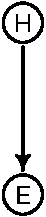
\includegraphics{conjunction-paradox4_files/figure-latex/fig:hEDAG-1} \end{center}
\begin{tabular}{c|cc}
& $H$ & $\neg H$ \\
\hline
$E$ & $\pr{E \vert H}$ & $\pr{E\vert \neg H}$ \\
$\neg E$ & $\pr{\neg E\vert H}$ & $\pr{\neg E\vert \neg H}$ \\
\end{tabular}

\caption{DAG of the simplest evidential relation along with a probability table}
\label{fig:hEDAG}
\end{wrapfigure}

\ali{M: Graphs are backwards, arrows go from hypothesis node to evidence nodes, hat is, 
from H to E and a to A and from B to b. Please fix.}

The simplest evidential relation, one of evidence bearing on a
hypothesis, can be represented by the directed graph displayed in Figure
\ref{fig:hEDAG}. The arrow need not have a causal interpretation. The
direction of the arrow indicates which conditional probabilities should
be supplied in the probability table. Since the arrow goes from \(H\) to
\(E\), we should specify the probabilities of the different values of
\(E\) conditional on the different values of \(H\).

Return now to the difficulty with conjunction. We will first examine the
case in which the two hypotheses \(A\) and \(B\) are probabilistically
independent. We will relax this assumption later. The two directed
graphs visualized in Figure \ref{fig:abBDAG} represent two items of
evidence each supporting its own hypothesis: \(a\) supports \(A\) and
\(b\) supports \(B\). To represent the conjunction \(A\wedge B\), a
conjunction node \(AB\) is added and arrows are drawn from nodes \(A\)
and \(B\) into node \(AB\) (Figure \ref{fig:conjunctionDAGchapter}).
This arrangement makes it possible to express the meaning of
\(A\wedge B\) via a probability table that mirrors the truth table for
the conjunction in propositional logic (see Table
\ref{tab:CPTconjunction}).\footnote{The difference is that the values
  \(1\) and \(0\) stand for two different things depending on where they
  are in the table. In the columns corresponding to the nodes they
  represent node states: true and false; in the \(\textsf{Pr}\) column
  they represent the conditional probability of a given state of \(AB\)
  given the states of \(A\) and \(B\) listed in the same row. For
  instance, take a look at row two. It says: if \(A\) and \(B\) are both
  in states 1, then the probability of \(AB\) being in state 0 is 0. In
  principle we could use `true' and `false' instead of 1 and 0 to
  represent states, but the numeric representation is easier to use in
  programming, which we do quite a bit in the background, so the reader
  might as well get used to this harmless ambiguity. For binary nodes,
  we will consistently use `1' and `0' for the states, it's just
  probabilities that in this case end up being extreme.}

\begin{figure}[h]
\begin{subfigure}[!ht]{0.45\textwidth}

\begin{center}
\includegraphics[width=0.6\linewidth]{conjunction-paradox4_files/figure-latex/fig:aADAG-1} \end{center}
\end{subfigure}\begin{subfigure}[!ht]{0.45\textwidth}

\begin{center}
\includegraphics[width=0.6\linewidth]{conjunction-paradox4_files/figure-latex/fig:bBDAG-1} \end{center}
\end{subfigure}
\caption{\textsf{DAG}s of $a$ supporting $A$ and $b$ supporting $B$.}
\label{fig:abBDAG}
\end{figure}

\begin{figure}[H]

\begin{center}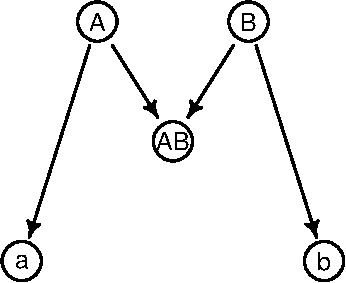
\includegraphics[width=0.6\linewidth]{conjunction-paradox4_files/figure-latex/fig:conjunctionDAG-1} \end{center}

\caption{\textsf{DAG} of the conjunction set-up, with the usual independence assumptions built in (\textsf{DAG 1}).}
\label{fig:conjunctionDAGchapter}
\end{figure}

\pagebreak 
\begin{wraptable}{l}{0.4\textwidth}
\begin{tabular}{lllr}
\toprule
\multicolumn{1}{c}{} & \multicolumn{1}{c}{A} & \multicolumn{1}{c}{B} & \multicolumn{1}{c}{} \\
AB &  &  & Pr\\
\midrule
\cellcolor{gray!6}{1} & \cellcolor{gray!6}{1} & \cellcolor{gray!6}{1} & \cellcolor{gray!6}{1}\\
0 & 1 & 1 & 0\\
\cellcolor{gray!6}{1} & \cellcolor{gray!6}{0} & \cellcolor{gray!6}{1} & \cellcolor{gray!6}{0}\\
0 & 0 & 1 & 1\\
\cellcolor{gray!6}{1} & \cellcolor{gray!6}{1} & \cellcolor{gray!6}{0} & \cellcolor{gray!6}{0}\\
0 & 1 & 0 & 1\\
\cellcolor{gray!6}{1} & \cellcolor{gray!6}{0} & \cellcolor{gray!6}{0} & \cellcolor{gray!6}{0}\\
0 & 0 & 0 & 1\\
\bottomrule
\end{tabular}

\caption{Conditional probability table for the conjunction node.}
\label{tab:CPTconjunction}
\end{wraptable}

The resulting graph, call it \textsf{DAG 1}, satisfies the desired
independence assumptions. First, the two claims \(A\) and \(B\) are
probabilistically independent of one another. Their independence is
guaranteed by the fact that the conjunction node \(AB\) is a collider
and thus no information flows through it.\footnote{A more formal
  treatment of this point is provided in
  \textbf{REFER TO OTHER CHAPTER}.} Second, the supporting items of
evidence \(a\) and \(b\) are also probabilistically independent of one
another. The reason is the same: node \(AB\) blocks any flow of
information between the evidence nodes. Notably, the independence of the
items of evidence is not always explicitly stated in the formulation of
the conjunction paradox. The good thing is that the Bayesian network
makes this assumption explicit.

With this set-up in place, the conjunction paradox arises because
aggregation is violated. By the theory of Bayesian networks,
\textsf{DAG 1} in Figure \ref{fig:conjunctionDAGchapter}

ensures the following:\footnote{This is because the only path between
  \textsf{A} and \textsf{B} goes through \textsf{AB}, which is a
  collider; as long as we do not condition on it, all paths between
  \textsf{A} and \textsf{B} remain blocked. See our chapter introducing
  Bayesian networks for details on this issue.
  \textbf{REFER TO APPROPRIATE CHAPTER}} \begin{align*}
\pr{A \wedge  B \vert a \wedge b}& =\pr{A \vert a \wedge b} \times \pr{B \vert  a \wedge b \wedge A}\\
 & = \pr{A \vert a} \times \pr{B \vert  b}
 \end{align*}

\noindent Thus, even when claims \(A\) and \(B\) are sufficiently
probable given their supporting evidence \(a\) and \(b\) (for a fixed
threshold \(t\))---in symbols, \(\pr{A \vert a}>t\) and
\(\pr{B \vert b}>t\)---it does not generally follow that \(A \et B\) is
sufficiently probable given combined evidence \(a\et b\) provided (as is
normally the case) neither \(\pr{A \vert a}\) nor \(\pr{B \vert b}\)
equal 1. As before, the conjunction principle fails because aggregation
fails.

The argument here goes beyond the specific example about aggravated
assault in the previous section. The argument only assumes that the
directed graph in Figure \ref{fig:conjunctionDAGchapter} is an adequate
representation of a situation in which two items of evidence, \(a\) and
\(b\), support their own hypothesis, \(A\) and \(B\). The graph encodes
two plausible relations of probabilistic independence: between
hypotheses \(A\) and \(B\) and between items of evidence \(a\) and
\(b\). The theory of Bayesian networks does the rest of the work.

\hypertarget{dependent-hypotheses}{%
\subsection{Dependent hypotheses}\label{dependent-hypotheses}}

Consider now what happens if claims \(A\) and \(B\) are not regarded as
probabilistically independent. To represent this, it is enough to draw
an arrow between nodes \(A\) and \(B\). The modified graph is displayed
in Figure \ref{fig:conjunctionDAG2chapter}, call it \textsf{DAG 2}. The
open path between nodes \(A\) and \(B\) no longer guarantees the
probabilistic independence of \(A\) and \(B\) or the independence of
evidence nodes \(a\) and \(b\). Note, however, that there is still no
\emph{direct} dependence between the items of evidence. The items of
evidence are still probabilistically independent of one another
\textit{conditional} on their respective hypothesis. That is,
\(\pr{a \vert A}=\pr{a \vert A \wedge b}\) and
\(\pr{b \vert B}=\pr{b \vert B \wedge a}\). So \(a\) and \(b\) still
count as independent lines of evidence despite not being
(unconditionally) probabilistically independent.\footnote{Here is an
  illustration of the idea of independent lines of evidence without
  unconditional independence. Suppose the same phenomenon (say blood
  pressure) is measured by two instruments. The reading of the two
  instruments (say `high' blood pressure) should be
  \textit{probabilistically dependent} of one another. After all, if the
  instruments were both infallible and they were measuring the same
  phenomenon, they should give the exact same reading. On the other
  hand, the two instruments measuring the same phenomenon should count
  as \textit{independent lines of evidence}. This fact is rendered in
  probabilistic terms by means of probabilistic independence conditional
  on the hypothesis of interest. These ideas can be worked out more
  systematically in the language of Bayesian networks. Roughly, two
  variables are probabilistically dependent if there is an open path
  between them. On the other hand, an open path can be closed by
  conditioning on one of the variables along the path. For a more
  rigorous exposition of the notions of open and closed paths, see
  \textbf{CITE EARLIER CHAPTERS}.}

\begin{figure}[h]

\begin{center}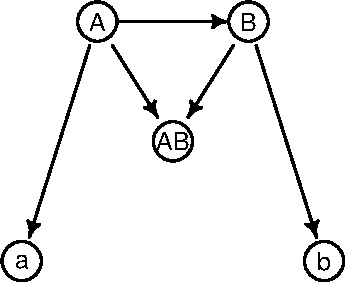
\includegraphics[width=0.6\linewidth]{conjunction-paradox4_files/figure-latex/fig:conjunctionDAG2-1} \end{center}
\caption{\textsf{DAG} of the conjunction set-up, without independence between $A$ and $B$ (\textsf{DAG 2}).}
\label{fig:conjunctionDAG2chapter}
\end{figure}

The difficulty with conjunction arises even without the independence of
hypotheses \(A\) and \(B\), at least in a number of circumstances. To
see why this is the case analytically is a bit cumbersome (see appendix
for details).
\raf{M: I think we should move the analytical arguemnt to the appendix or remove it entirely. It's muddled. Commented it out}
But we can study how often, in principle, the joint posterior
\(\pr{A\wedge B \vert a \wedge b}\) is below both of the individual
posteriors \(\pr{A \vert a}\) and \(\pr{B \vert b}\). To this end, we
simulated 10,000 random Bayesian networks based on \textsf{DAG 1} and
\textsf{DAG 2}. Assuming that each possible Bayesian network has an
equal probability of occurring, the joint posterior is lower than both
individual posteriors 68\% of the time for \textsf{DAG 1}, and around
60\% for \textsf{DAG 2} (see the appendix for details). This result
agrees with Schwartz \& Sober (2017) who pointed out that, if hypotheses
\(A\) and \(B\) are probabilistically dependent on one another,
aggregation will fail less often. Still, postulating a dependence
between hypotheses does little for solving the difficulty with
conjunction since a drop in the failure rate from 68\% to 60\% is
limited.

\vspace{1mm}
\footnotesize

\normalsize

\hypertarget{evidential-strength}{%
\section{Evidential Strength}\label{evidential-strength}}

\label{sec:strength}

The previous section demonstrated that aggregation fails in a large
class of cases if the standard of proof is understood as a posterior
probability threshold. Some believe that such failures are strong enough
ground to advocate a different conception of probability, along the
lines of Baconian probability (L. J. Cohen, 2008), fuzzy logic or belief
functions (Clermont, 2013), or reject legal probabilism altogether
(Allen \& Stein, 2013). But posterior probability thresholds are not the
only way of understanding standards of proof from a probabilistic
perspective. Standards of proof can also be modeled using probabilistic
measures of \textit{evidential strength}. This is the approach we
explore in this section.

Two common probabilistic measures of evidential strength are the Bayes
factor and the likelihood ratio. We discussed them earlier in Chapter
XX. \todo{REFER TO EARLIER CHAPTERS} As we show below, under plausible
assumptions, these measures of evidential strength validate one
direction of the conjunction principle: aggregation. If \(a\) is
sufficiently strong evidence in favor of \(A\) and \(b\) is sufficiently
strong evidence in favor of \(B\), then \(a\wedge b\) is sufficiently
strong evidence in favor of the conjunction \(A \wedge B\). In fact, the
evidential support for the conjunction will often exceed that for the
individual claims, a point already made by Dawid (1987) who wrote that
`suitably measured, the support supplied by the conjunction of several
independent testimonies exceeds that supplied by any of its
constituents' (97).

Dawid thought that vindicating aggregation was enough for the
conjunction paradox to `evaporate.' But, as we show below, this is not
quite right. On the evidential strength interpretation of the standard
of proof, the other direction of the conjunction principle,
distribution, fails. If \(a \wedge b\) is sufficiently strong evidence
in favor of \(A \wedge B\), it does not follow that \(a\wedge b\) is
sufficiently strong evidence in favor of \(A\) or that \(a\wedge b\) is
sufficiently strong evidence in favor of \(B\). This is odd. If we
interpret the standard of proof using evidential strength, one could
establish beyond a reasonable doubt that \(A \wedge B\) (say the
defendant killed the victim \textit{and} acted intentionally) while
failing to establish one of the conjuncts.

The prospects for legal probabilism look dim. If the standard of proof
is understood as a posterior probability threshold, the conjunction
principle fails because aggregation fails (previous section). If,
instead, the standard of proof is understood as a threshold relative to
evidential strength, the conjunction principle still fails because
distribution fails (this section). From a probabilistic perspective, it
seems impossible to capture both directions of the conjunction
principle. In what follows, we defend more precisely the claim that, on
the evidential strength approach, aggregation succeeds but distribution
fails. The argument is laborious. The reader should arm themselves with
patience or take our word for it and jump ahead. The curious reader is
welcome to read the appendix for the technical details.

\hypertarget{combined-support-bayes-factor}{%
\subsection{Combined support: Bayes
factor}\label{combined-support-bayes-factor}}

The first part of the argument shows that the combined support supplied
by multiple pieces of evidence (e.g.~\(a\wedge b\)) for a conjunctive
claim (e.g.~\(A\wedge B\)) typically exceeds the individual support
supplied by individual pieces of evidence for individual claims. This
claim holds for the Bayes factor and to some extent for the likelihood
ratio. We start with the Bayes factor \(\pr{E \vert H}/\pr{E}\) as our
measure of the support of \(E\) in favor of \(H\). As is apparent from
Bayes' theorem,

\[\pr{H \vert E} = \frac{\pr{E \vert H}}{\pr{E}}\times \pr{H},\]

\noindent the Bayes factor measures the extent to which a piece of
evidence increases the probability of a hypothesis, as compared to its
prior probability. The greater the Bayes factor (for values above one),
the stronger the support of \(E\) in favor of \(H\).

Suppose Bayes factors \(\nicefrac{\pr{a \vert A}}{\pr{a}}\) (abbreviated
\(BF_A\)) and \(\nicefrac{\pr{b \vert B}}{\pr{b}}\) (abbreviated
\(BF_B\)) are greater than one. That is, items of evidence \(a\) and
\(b\) positively support \(A\) and \(B\), separately. The combined
support here is (see the appendix for a proof): \begin{align*}
\frac{\pr{a \wedge b \vert A \wedge B}}{\pr{a \wedge b}} &= \frac{\pr{a \vert A}}{\pr{a}} \times \frac{\pr{b \vert B}}{\pr{b}}\\
BF_{AB} &= BF_{A} \times BF_{B}
\end{align*} \noindent Consequently, the combined support \(BF_{AB}\) is
always higher than the individual support so long as the individual
pieces of evidence positively support their respective hypothesis. This
claim holds assuming hypotheses \(A\) and \(B\) are independent and
items of evidence \(a\) and \(b\) are independent. These assumptions are
validated by \textsf{DAG 1} in Figure \ref{fig:conjunctionDAGchapter}.
Under these circumstances, Dawid's claim that `the support supplied by
the conjunction of several independent testimonies exceeds that supplied
by any of its constituents' (if support is to be measured in terms of
Bayes factor) is verified.\footnote{The result holds beyond two pieces
  of evidence; see Figure \ref{fig:bfconjunction5}). Note that the order
  is reversed if the items of evidence oppose the individual hypotheses.
  Neutral evidence results in a combined Bayes factor of 1, no matter
  the prior or the number of items of evidence.}

\ali{R: recode lty scale so that the order is five-two-one in the legend.}
\begin{figure}[h]

\begin{center}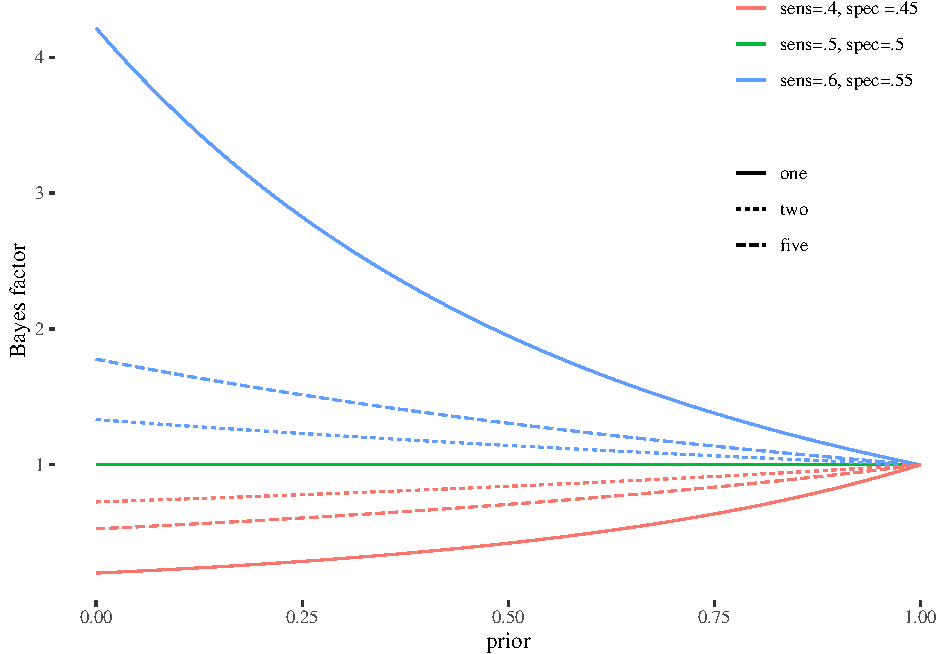
\includegraphics[width=0.9\linewidth]{conjunction-paradox4_files/figure-latex/bfconjunction5-1} \end{center}
\caption{Bayes factor for one, two and five items of evidence and the corresponding claims, given different degrees of specificity and sensitivity of the evidence. The independence assumptions in Figure \ref{fig:conjunctionDAGchapter}, \textsf{DAG 1}, hold.}
\label{fig:bfconjunction5}
\end{figure}

Even when \(A\) and \(B\) are not probabilistically independent, the
combined Bayes factor \(BF_{AB}\) will still be greater than both the
individual Bayes factor \(BF_{A}\) and \(BF_{B}\) if the probabilistic
measure fits \textsf{DAG 2} in Figure \ref{fig:conjunctionDAG2chapter}.
To see why, first note that the following holds (see the appendix for a
proof):

\begin{align}
BF_{AB}&= \frac{\pr{a \wedge b\vert A\wedge B}}{\pr{a \wedge b}}&= \frac{\pr{a |A}}{\pr{a}} \times \frac{\pr{b |B}}{\pr{b|a}}&=  BF_{A}\times BF^{'}_{B} \nonumber \\
& & = \frac{\pr{a |A}}{\pr{a | b}} \times \frac{\pr{b |B}}{\pr{b}}& =  BF^{'}_{A}\times BF_{B}  \nonumber 
 \end{align}

\noindent The difference from the case of independent hypotheses is that
\(BF_B=\nicefrac{\pr{b \vert B}}{\pr{b}}\) is now replaced by
\(BF^{'}_B=\nicefrac{\pr{b \vert B}}{\pr{b\vert a}}\), or alternatively
\(BF_A=\nicefrac{\pr{a \vert A}}{\pr{a}}\) by
\(BF^{'}_A=\nicefrac{\pr{a \vert A}}{\pr{a\vert b}}\).\footnote{Since
  \(b\) need not be probabilistically independent of \(a\), there is no
  guarantee that \(\pr{b \vert a}=\pr{b}\) or \(\pr{a \vert b}=\pr{a}\).}
Still, if the probabilistic measure fits \textsf{DAG 2}, whenever
\(BF_B\) is greater than 1, so is \(BF^{'}_B\), and whenever \(BF_A\) is
greater than 1, so is \(BF^{'}_A\) (see the appendix for a proof). Thus,
the joint Bayes factor \(BF_{AB}\) will be greater than any of the
individual Bayes factors.\footnote{In contrast, if the underlying
  \textsf{DAG} were to contain a direct dependence between the items of
  evidence, the joint Bayes factor could be lower than either of the
  individual Bayes factors (see the appendix for a proof).}

\hypertarget{combined-support-likelihood-ratio}{%
\subsection{Combined support: likelihood
ratio}\label{combined-support-likelihood-ratio}}

We now run a similar argument for the likelihood ratio, another
probabilistic measure of evidential strength. The likelihood
ratio---extensively discussed in Chapter XX
\todo{REFER TO EARLIER CHAPTER}---compares the probability of the
evidence on the assumption that a hypothesis of interest is true
(\textit{sensitivity}) and the probability of the evidence on the
assumption that the negation of the hypothesis is true
(\textit{1- specificity}). That is,
\[\frac{\pr{E \vert H}}{\pr{E \vert \neg H}}=\frac{\textit{sensitivity}}{\textit{1- specificity}}\]

\noindent The greater the likelihood ratio (for values above one), the
stronger the evidential support in favor of the hypothesis (as
contrasted to its negation).

The question is whether the combined support measured by the combined
likelihood ratio
\[\frac{\pr{a\wedge b \vert A\wedge B}}{\pr{a \wedge b \vert \neg (A\wedge B)}}\]

\noindent exceeds the individual support measured by the individual
likelihood ratios \(\nicefrac{\pr{a \vert A}}{\pr{a \vert \neg A}}\) and
\(\nicefrac{\pr{b \vert B}}{\pr{b \vert \neg B}}\). Under suitable
assumptions, the answer is positive. So, details aside, Bayes factor and
likelihood ratio agree here. The argument for the likelihood ratio,
however, is more laborious.

We start with the fact that, in a large class of cases (see the appendix
for a proof),

\begin{align*}
LR_{AB} & = \frac{\pr{a\wedge b \vert A\wedge B}}{\pr{a \wedge b \vert \neg (A\wedge B)}} = \frac{\pr{a \vert A} \times \pr{b \vert B}}
 {\frac{\pr{\neg A}\pr{B \vert \neg A} \pr{a \vert \neg A}\pr{b \vert B} + \pr{A}\pr{\neg B \vert A} \pr{a \vert A }\pr{b \vert \neg B} + \pr{\neg A}\pr{\neg B \vert \neg A } \pr{a \vert \neg A}\pr{b \vert \neg B}}{\pr{\neg A}\pr{B \vert \neg A} + \pr{A}\pr{\neg B \vert A } + \pr{\neg A}\pr{\neg B \vert \neg A} }}
\end{align*}

\noindent This equality is general. It holds whether or not hypotheses
\(A\) and \(B\) are probabilistically independent. Given the many
unknowns here, it pays to make some simplifications if only for
illustrative purposes.

The first simplification we make is to assume that the sensitivity and
specificity of the items of evidence are both equal to the same value
\(x\). Second, we assume that \(A\) and \(B\) are probabilistically
independent in agreement with \textsf{DAG 1} (Figure
\ref{fig:conjunctionDAGchapter}). The combined likelihood ratio can now
be plotted as a function of \(x\). Figure \ref{fig:jointLRMarcello}
shows that the combined likelihood ratio always exceeds the individual
likelihood ratios whenever they are greater than one (or in other words,
as is usually assumed, the two pieces of evidence provide positive
support for their respective hypotheses).\footnote{Interestingly, the
  combined likelihood ratio varies depending on the prior probabilities
  \(\pr{A}\) and \(\pr{B}\).} As with the Bayes factor, the combined
likelihood ratio exceeds the individual likelihood ratios.

\begin{figure}

\begin{center}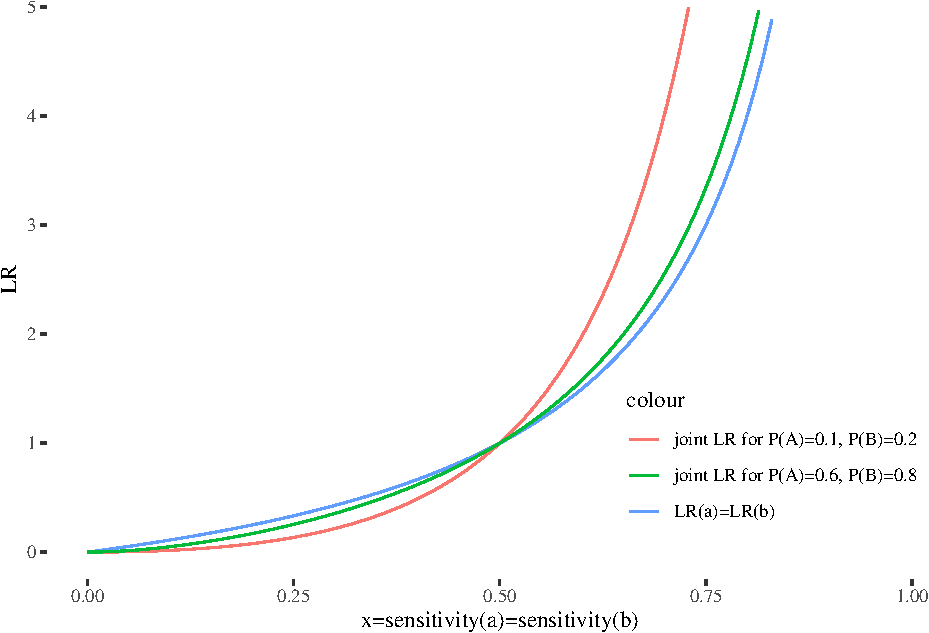
\includegraphics[width=0.9\linewidth]{conjunction-paradox4_files/figure-latex/unnamed-chunk-3-1} \end{center}

\caption{Combined likelihood ratios exceeds individual Likelihood ratios as soon as sensitivity is above .5. Changes in the prior probabilities $\pr{A}$ and $\pr{B}$ do not invalidate this result.}
\label{fig:jointLRMarcello}
\end{figure}

What happens if the two simplifying assumptions are relaxed? If the
items of evidence have different levels of sensitivity and specificity,
the combined likelihood ratio never goes below the lower of the two
individual likelihood ratios, but can be lower than the higher
individual likelihood ratio. We established this claim by means of a
computer simulation (see the appendix for details). This holds if the
probabilistic measure fits \textsf{DAG 1} (independent hypotheses) or
\textsf{DAG 2} (dependent hypotheses), but fails if there is direct
dependence between the pieces of evidence.\footnote{The simplified
  set-up from before does not contradict this claim but follows from it.
  In the simplified set-up, both individual likelihood ratios were the
  same, so whenever the joint likelihood was higher than the minimum of
  the individual likelihood ratios, it was higher than the both of them.}
In this sense, the joint likelihood ratio behaves differently than the
joint Bayes factor since it is greater than the lowest of the individual
likelihood ratios, rather than being greater than both of them.
Consequently, Dawid's claim that `the support supplied by the
conjunction of several independent testimonies exceeds that supplied by
any of its constituents' should be weakened. The evidential support
(when it is measured by the likelihood ratio) supplied by the
conjunction of several independent items of evidence exceeds the support
supplied by at least one individual item of evidence but possibly not
all.

\hypertarget{vindicating-aggregation}{%
\subsection{Vindicating aggregation}\label{vindicating-aggregation}}

We have seen that under suitable assumptions the combined evidential
support is never below the lowest individual support. More precisely,
let \(\mathsf{str}[E, H]\) stand for the strength of the evidential
support of a piece of evidence \(E\) toward a hypothesis \(H\), measured
by the Bayes factor or the likelihood ratio. We have established the
following fact:

\[\mathsf{str}[a \wedge b, A\wedge B] \geq \text{min}(\mathsf{str}[a, A], \mathsf{str}[b, B]),\]
where the function \(\text{min}\) returns the lowest of its arguments.

This fact can be used to justify aggregation. To be sure, aggregation is
not directly a principle about evidential strength. It is a principle
about the standard of proof. So, to complete the argument, the standard
of proof should be tied to evidential strength. How? The rule of
decision could be: liability is proven according to the governing
standard of proof in case the strength of the evidential
support---measured by the Bayes factor or the likelihood ratio---meets a
suitably high threshold. On this reading, the threshold should no longer
be a posterior probability between 0 and 1, but a number somewhere above
one. The greater this number, the more stringent the standard of proof,
for any value above one.

The only question left at this point is, how to identify the appropriate
evidential strength threshold? The answer isn't obvious. Below we
examine two possible approaches. First, the threshold for the Bayes
factor and the threshold for the likelihood ratio can be derived from
the threshold for the posterior probability by manipulating two simple
equations. Consider first the Bayes factor threshold. Since
\begin{align*}
\mathsf{ Bayes \: factor }=\frac{\mathsf{posterior }}{\mathsf{ prior}},
\end{align*}

\noindent the Bayes factor threshold, call it \(t_{BF}\), can be defined
as follows: \begin{align*}t_{BF} & = \frac{t}{\textsf{prior}},
\end{align*} where \(t\) is the posterior probability threshold. The
value of \(t\) can be determined in a decision-theoretic manner by
minimizing expected costs (see Chapter XX
\todo{REFER TO ERALIER CHAPPER}). Once \(t\) is fixed in this way, the
value \(t_{BF}\) can be easily derived by the equations above. The same
strategy works for the likelihood ratio threshold, call it \(t_{LR}\).
By the odds version of Bayes' theorem,
\begin{align*}\textsf{likelihood ratio}=\frac{\textsf{posterior odds}}{\textsf{prior odds}}.
\end{align*} If the posterior ratio is fixed at, say \(t/1-t\), then the
value of \(t_{LR}\) can be easily obtained as follows:
\begin{align*}t_{LR} & = \frac{\nicefrac{t}{1-t}}{\textsf{prior odds}}.
\end{align*}

\noindent Note that thresholds \(t_{BF}\) and \(t_{LR}\) will depend on
the prior probability of the hypothesis. The higher the prior
probability, the lower the threshold. Whether this is a desirable
property of a decision threshold can be questioned, but a similar point
applies to the posterior threshold \(t\): the higher the prior
probability, the easier to meet the threshold.

This approach is simple and elegant, but incurs a major shortcoming:
aggregation still fails. There will be cases in which the conjuncts
taken separately satisfy the decision standard \(t_{BF}\) or \(t_{LR}\),
while the conjunction does not.
\raf{Question: how does Kaplow think about it? Does he only derive threshold for the ultimate claim? I don't remember now.}
To illustrate, consider a posterior probability threshold of \(.95\) as
might be appropriate in a criminal case. If the individual claims \(A\)
and \(B\) both have a prior probability of, say \(.1\), the Bayes factor
threshold \(t^A_{BF}=t_{BF}^B=\nicefrac{.95}{.1}=9.5\) for \(A\) or
\(B\) individually. Note the superscripts \(A\) and \(B\). The Bayes
factor threshold \(t_{BF}\) is indexed to the claim of interest because
the threshold is prior-dependent and thus claim-dependent (since
different claims have different prior probabilities). If, as is often
assumed, claims \(A\) and \(B\) are probabilistically independent, the
composite claim \(A \wedge B\) will be associated with the Bayes factor
threshold \(t^{A\wedge B}_{BF}=\nicefrac{.95}{(.1\times .1)}=95\), a
much higher value. Suppose each claim barely meet the 9.5 Bayes factor
threshold. Given independence, the joint Bayes factor results from
multiplying the individual Bayes factors, that is,
\(9.5 \times 9.5=90.25\). This is not quite enough to meet
\(t^{A\wedge B}_{BF}=95\). So aggregation fails. An analogous point
holds for the likelihood ratio threshold.\footnote{Say \(A\) and \(B\)
  have prior probabilities of \(.2\) and \(.3\) respectively. On this
  approach, the likelihood ratio threshold for \(A\) and \(B\) will be
  \(t_{LR}^{A}\approx 76\) and \(t_{LR}^{B}a\approx 44\), assuming
  posterior probability threshold of 0.95. The likelihood ratio
  threshold for the composite claim \(A \wedge B\) will be
  \(t^{A\wedge B}_{LR}\approx 297\). Suppose the individual likelihood
  ratios meet their threshold. And, for simplicity, suppose sensitivity
  and specificity of the individual items of supporting evidence are the
  same. In this case, for \(t_{LR}^{A}\) to be met, evidence \(a\)
  should have sensitivity (and specificity) of at least 0.988. For
  \(t_{LR}^{B}\) to be met, evidence \(b\) should have sensitivity (and
  specificity) of 0.978. Given these values, the combined likelihood
  ratio equals about 145, far short from the threshold
  \(t^{A\wedge B}_{LR}\approx 297\).} The culprit is the fact that
\(t_{BF}\) and \(t_{LR}\) have different values when applied to
individual claims \(A\) and \(B\) as opposed to the composite claim
\(A \wedge B\).

But not all hope is lost. Perhaps it is unsurprising that deriving the
evidential strength threshold from the posterior probability threshold
did not solve the problem. If there are reasons to reject the posterior
probability threshold, these reasons also apply to thresholds that are
parasitic to it. The second approach we consider is more
straightforward. It consists in fixing the evidential strength threshold
independently of the posterior probability threshold and regardless of
the the prior probability of the hypothesis. Criminal cases would still
have a higher decision threshold than civil cases, but the threshold
would be constant across individual and composite claims.\footnote{ This
  approach raises the question of how the threshold should be fixed in
  the first place. Since the threshold is no longer derived from the
  posterior probability threshold, standard decision theory cannot help
  here. We do not further examine this question, since this approach is
  not part of our ultimate solution to the conjunction paradox.} The
good news is that the fixed threshold approach vindicates aggregation.
The argument is easy. As seen previously, the combined evidential
support is usually greater than at least one, if not all, individual
evidential supports, whether measured by the Bayes factor or the
likelihood ratio. So, for a fixed value of the threshold, whenever
\(BF_A\) and \(BF_B\) meet the threshold \(t_{BF}\), usually also the
combined Bayes factor \(BF_{AB}\) meets \(t_{BF}\). The same applies for
the likelihood ratio threshold. Whenever \(LR_A\) and \(LR_B\) meet the
threshold \(t_{LR}\), then usually also \(LR_{AB}\) meets \(t_{LR}\).
Aggregation is finally vindicated!

\hypertarget{the-failure-of-distribution}{%
\subsection{The failure of
distribution}\label{the-failure-of-distribution}}

But it is too soon to declare victory. The trouble is that, if the
evidential strength threshold is held fixed across individual and
composite claims, the principle of distribution becomes problematic.
This is the other direction of the conjunction principle. Distribution
posits that establishing the conjunction, by a governing standard of
proof, is sufficient for establishing the individual conjuncts. This is
a seemingly uncontroversial principle. How can it possibly fail? To be
clear, the principle of distribution does not fail if the standard of
proof is understood as a posterior probability threshold. After all, the
probability of a conjunction cannot be higher than the probability of
its conjuncts. But distribution does fail if the standard of proof is
understood as an evidential strength threshold.

For suppose the combined Bayes factor,
\(\nicefrac{\pr{a \et b \vert A \et B}}{\pr{a \et b}}\), barely meets
the threshold. The individual support, say
\(\nicefrac{\pr{a \vert A}}{\pr{a}}\), could still be below the
threshold unless \(\nicefrac{\pr{b \vert B}}{\pr{b}}=1\) (which should
not happen if \(b\) positively supports \(B\)). The problem for
likelihood ratio is analogous. Looking at the graphs in Figure
\ref{fig:bfconjunction5} and Figure \ref{fig:jointLRMarcello} should be
enough to convince oneself that this is the case. So---if the standard
of proof is interpreted as a fixed evidential strength threshold---even
though the conjunction \(A \et B\) was proven according to the desired
standard, one of the individual claims might not.

We have just shown that the following distribution principles fails:
\begin{align}
S[a \wedge b, A\wedge B] \Rightarrow S[a, A] \wedge S[b, B], \tag{DIS1}
\end{align} where \(S\) is a placeholder for the standard of proof. But,
perhaps, principle (DIS1) is not as obviously intuitive as one might
have thought. Since the evidence is not held constant throughout, the
support supplied by \(a\wedge b\) could be stronger than that supplied
by \(a\) and \(b\) individually. After all, the individual evidence
\(a\) or \(b\) is weaker evidence than the combined evidence
\(a\wedge b\). At least one might argue this way.

To accommodate this line of reasoning, here is a weaker distribution
principle: \begin{align}
S[a \wedge b, A\wedge B] \Rightarrow S[a \wedge b, A] \wedge S[a\wedge b, B]. \tag{DIS2}
\end{align}

\noindent This principle is less controversial because it holds the
evidence constant. One would not want to claim that, while holding fixed
evidence \(a\wedge b\), establishing the conjunction might not be enough
for establishing one of the conjuncts. Yet, if \(A\) and \(B\) are
probabilistically independent, (DIS1) and (DIS2) are in fact equivalent
principles so long as the standard of proof is interpreted as a fixed
evidential strength threshold (see appendix for
details).\raf{M: Need proof of this. Is it in the appendix?} So the
counterexamples to the first distribution principle also work against
the weaker version.

\hypertarget{the-comparative-strategy}{%
\section{The comparative strategy}\label{the-comparative-strategy}}

\label{sec:comparative}

We hit two dead ends. The posterior probability threshold is subject to
the difficulty with conjunction, specifically, the failure of
aggregation (Section \ref{sec:difficulty}). The evidential strength
threshold is subject to another kind of difficulty, the failure of
distribution (Section \ref{sec:strength}). As a third approach, the
standard of proof can be understood comparatively. This approach has
been advanced by Cheng (2012) following the theory of relative
plausibility by Pardo \& Allen (2008). Say the prosecutor or the
plaintiff puts forward a hypothesis \(H_p\) about what happened. The
defense offers an alternative hypothesis, call it \(H_d\). On this
approach, rather than directly evaluating the support of \(H_p\) given
the evidence and comparing it to a threshold, we compare the support
that the evidence provides for two competing hypotheses \(H_p\) and
\(H_d\), and decide for the one that garners greater evidential support.

It is controversial whether this is what happens in all trial
proceedings, especially in criminal trials, if one thinks of the defense
hypothesis \(H_d\) as a substantial account of what has happened. The
defense may elect to challenge the hypothesis put forward by the other
party without proposing one of its own. In the O.J.~Simpson trial, for
example, the defense did not advance its own story about what happened,
but simply argued that the evidence provided by the prosecution, while
significant on its face to establish OJ's guilt, was riddled with
problems and deficiencies. This defense strategy was enough to secure an
acquittal. So, in order to create a reasonable doubt about guilt, the
defense does not always provide a full-fledged alternative hypothesis.
The supporters of the comparative approach, however, respond that this
could happen in a small number of cases, even though in
general---especially for tactical reasons---the defense will provide an
alternative hypothesis.

\hypertarget{comparing-posteriors}{%
\subsection{Comparing posteriors}\label{comparing-posteriors}}

Setting aside these qualms, we first work out the comparative strategy
using posterior probabilities. Here, the standard of proof is understood
as follows: given a body of evidence \(E\) and two competing hypotheses
\(H_p\) and \(H_d\), the probability \(\pr{H_p \vert E}\) should be
suitably higher than \(\pr{H_d \vert E}\), or in other words, the ratio
\(\nicefrac{\pr{H_p \vert E}}{\pr{H_d \vert E}}\) should be above a
suitable threshold. Presumably, the ratio threshold should be higher for
criminal than civil cases, for example, greater than one for civil cases
and substantively above one for criminal cases.\footnote{In the
  comparative approach---as Cheng (2012) shows---expected utility theory
  can set the appropriate threshold as a function of the costs and
  benefits of trial decisions. Suppose the costs of a false positive is
  \(c_{FP}\) and that of a false negative is \(c_{FN}\), both greater
  than zero. Intuitively, the decision rule should minimize the expected
  costs (see Chapter YYY). That is, a finding against the defendant
  would be acceptable whenever its expected
  costs---\(\pr{H_d \vert E} \times c_{FP}\)---are smaller than the
  expected costs of an
  acquittal---\(\pr{H_p \vert E}\times c_{FN}\)---or in other words:
  \(\frac{\pr{H_p \vert E}}{\pr{H_d \vert E}} > \frac{c_{FP}}{c_{FN}}\).
  In civil cases, it is customary to assume the costs ratio of false
  positives to false negatives equals one. So the rule of the decision
  would be: find against the defendant whenever \(\pr{H_p \vert E}\) is
  greater than \(\pr{H_d \vert E}\). In criminal trials, the costs ratio
  is considered higher, since convicting an innocent (false positive)
  should be more harmful or morally objectionable than acquitting a
  guilty defendant (false negative). So the rule of decision would be:
  convict whenever \(\pr{H_p \vert E}\) is substantively greater than
  \(\pr{H_d \vert E}\).} Note that \(H_p\) and \(H_d\) need not be one
the negation of the other.\footnote{If two hypotheses are exclusive and
  exhaustive, \(\nicefrac{\pr{H_p \vert E}}{\pr{H_d \vert E}}>1\)
  implies that \(\pr{H_p \vert E}>.5\), the standard probabilistic
  interpretation of the preponderance standard for civil cases, and
  \(\nicefrac{\pr{H_p \vert E}}{\pr{H_d \vert E}}>19\) implies that
  \(\pr{H_p \vert E}>.95\), a common interpretation of proof beyond a
  reasonable doubt.}

We will work through a stylized case used by Cheng himself. Suppose, in
a civil case, the plaintiff claims that the defendant was speeding
(\(S\)) and that the crash caused her neck injury (\(C\)). Here the
plaintiff's hypothesis is \(S\et C\). Suppose, given evidence \(E\), the
conjuncts, taken separately, meet the decision threshold: \begin{align}
 \nonumber 
 \frac{\pr{S\vert E}}{\pr{\neg S \vert E}} > 1   & & \frac{\pr{C\vert E}}{\pr{\neg C \vert E}} > 1
\end{align} \noindent To see whether aggregation is satisfied, we check
whether \(\nicefrac{\pr{S\et C\vert E}}{\pr{H_d \vert E}}>1\). The key
is to decide on the defense hypothesis \(H_d\). Cheng reasons that there
are three alternative defense scenarios: \(H_{d_1}= S\et \n C\),
\(H_{d_2}=\n S \et C\), and \(H_{d_3}=\n S \et \n C\). How does \(H_p\)
compare to each of them? Assuming independence between \(C\) and \(S\),
we have:\footnote{We are assuming that \(E\) is the conjunction of two
  items of evidence, \(s\et c\), where \(s\) supports \(S\) and \(c\)
  supports \(C\). The inequalities holds on \textsf{DAG 1} in Figure
  \ref{fig:conjunctionDAGchapter} after replacing \(A\) and \(a\) by
  \(S\) and \(s\), and \(B\) and \(b\) by \(C\) and \(c\), respectively.}

\begin{align}\label{eq:cheng-multiplication}
\frac{\pr{S\et C\vert E}}{\pr{S\et \n C\vert E}} & = \frac{\pr{S\vert E}\pr{C\vert E}}{\pr{S \vert E}\pr{\n C \vert E}}  =\frac{\pr{C\vert E}}{\pr{\n C \vert E}} > 1 \\
\nonumber
\frac{\pr{S\et C\vert E}}{\pr{\n S\et C\vert E}} & = \frac{\pr{S\vert E}\pr{C\vert E}}{\pr{\n S \vert E}\pr{C\vert E}}  = \frac{\pr{S\vert E}}{\pr{\n S \vert E}} > 1 \\
\nonumber
\frac{\pr{S\et C\vert E}}{\pr{\n S\et \n C\vert E}} & = \frac{\pr{S\vert E}\pr{C\vert E}}{\pr{\n S \vert E}\pr{\n C \vert E}}   > 1 
\end{align}

\noindent So, whatever the defense hypothesis, the plaintiff's
hypothesis is more probable. At least in this case, whenever the
elements of a plaintiff's claim satisfy the decision threshold, so does
their conjunction. The left-to-right direction of the conjunction
principle---what we are calling aggregation---has been vindicated, at
least for simple cases involving independence. Success.

What about the opposite direction, distribution? Distribution is not
generally satisfied. Suppose
\(\nicefrac{\pr{S\et C\vert E}}{\pr{H_d \vert E}}>1\), or in other
words, the combined hypothesis \(S \et C\) has been established by
preponderance of the evidence. The question is whether the individual
hypotheses have been established by the same standard, specifically,
whether \(\frac{\pr{C\vert E}}{\pr{\n C \vert E}} > 1\) and
\(\frac{\pr{S\vert E}}{\pr{\n S \vert E}} > 1\). If
\(\nicefrac{\pr{S\et C\vert E}}{\pr{H_d \vert E}}>1\), the combined
hypothesis is assumed to be more probable than any of the competing
hypotheses, in particular,
\(\nicefrac{\pr{S\et C\vert E}}{\pr{\neg S \et C \vert E}}>1\),
\(\nicefrac{\pr{S\et C\vert E}}{\pr{S \et \neg C \vert E}}>1\) and
\(\nicefrac{\pr{S\et C\vert E}}{\pr{\neg S \et \neg C \vert E}}>1\). We
have: \begin{align}\label{eq:cheng-multiplication-two}
1 < \frac{\pr{S\et C\vert E}}{\pr{S\et \n C\vert E}} & = \frac{\pr{S\vert E}\pr{C\vert E}}{\pr{S \vert E}\pr{\n C \vert E}}  =\frac{\pr{C\vert E}}{\pr{\n C \vert E}} \\
\nonumber
1 < \frac{\pr{S\et C\vert E}}{\pr{\n S\et C\vert E}} & = \frac{\pr{S\vert E}\pr{C\vert E}}{\pr{\n S \vert E}\pr{C\vert E}}  = \frac{\pr{S\vert E}}{\pr{\n S \vert E}}  \\
\nonumber
1 < \frac{\pr{S\et C\vert E}}{\pr{\n S\et \n C\vert E}} & = \frac{\pr{S\vert E}\pr{C\vert E}}{\pr{\n S \vert E}\pr{\n C \vert E}}   
\end{align}

\noindent In the first two cases, clearly, if the composite hypothesis
meets the threshold, so do the individual claims. But consider the third
case.
\(\nicefrac{\pr{S\vert E}\pr{C\vert E}}{\pr{\n S \vert E}\pr{\n C \vert E}}\)
might be strictly greater than
\(\nicefrac{\pr{C\vert E}}{\pr{\n C \vert E}}\) or
\(\nicefrac{\pr{S\vert E}}{\pr{\n S \vert E}}\). It is possible that
\(\nicefrac{\pr{S\vert E}\pr{C\vert E}}{\pr{\n S \vert E}\pr{\n C \vert E}}\)
is greater than one, while
either\(\nicefrac{\pr{C\vert E}}{\pr{\n C \vert E}}\) or
\(\nicefrac{\pr{S\vert E}}{\pr{\n S \vert E}}\) are not, say when they
are 3 and 0.5, respectively. Distribution fails. And the same problem
would arise with a more stringent threshold as might be appropriate in
criminal cases.

There is a more general problem with Cheng's comparative approach. Much
of the heavy lifting here is done by the strategic splitting of the
defense line into multiple scenarios. Suppose, for illustrative
purposes, \(\pr{H_p\vert E}=0.37\) and the probability of each of the
defense lines given \(E\) is \(0.21\). This means that \(H_p\) wins with
each of the scenarios. We should then find against the defendant. But
should we? Given the evidence, the accusation is likely to be false,
because \(\pr{\n H_p \vert E}=0.63\). The problem generalizes. If, as
here, we individualize scenarios by Boolean combinations of elements of
a case, the more elements, the more alternative scenarios into which
\(\n H_p\) needs to be divided. This normally would lead to lowering
even further the probability of each of them (because now
\(\pr{\n H_p}\) needs to be split between more scenarios). If we take
this approach seriously, the more elements a case has, the more at a
disadvantage the defense is. This seems undesirable.

\hypertarget{comparing-likelihoods}{%
\subsection{Comparing likelihoods}\label{comparing-likelihoods}}

Instead of posterior probabilities, likelihoods can also be compared.
The standard of proof would then be as follows: the ratio between
likelihoods \(\nicefrac{\pr{E \vert H_p}}{\pr{E \vert H_d}}\) should be
above a suitable threshold. Note that the posterior ratio
\(\nicefrac{\pr{H_p \vert E}}{\pr{H_d \vert E}}\) from before was
replaced by the likelihood ratio
\(\nicefrac{\pr{E \vert H_p}}{\pr{E \vert H_d}}\) where \(H_d\) and
\(H_p\), as before, need not be exhaustive hypotheses. In civil cases,
the likelihood ratio should perhaps be just be above 1, meaning that the
evidence supports \(H_p\) more strongly than it supports \(H_d\). In
criminal cases, the ratio should be several orders of magnitude above
one. This approach runs into the same problem as Cheng's. It cannot
justify distribution.

We do not provide all the details of the argument. The reasoning is
analogous. Consider the car crash example from before, where \(S\)
stands for the defendant's speeding, \(C\) stands for the statement that
the crash caused neck injury, and \(E\) stands for the total evidence.
The plaintiff's hypothesis \(H_p\) is \(S\et C\). Suppose
\(\nicefrac{\pr{E \vert S\et C}}{\pr{E \vert H_d}}>1\), or in other
words, the combined hypothesis \(S \et C\) has been established by
preponderance of the evidence. The question is whether the individual
hypotheses have been established by the same standard, specifically,
whether \(\frac{\pr{E \vert C}}{\pr{E\vert \neg C}} > 1\) and
\(\frac{\pr{E \vert S}}{\pr{E\vert \neg S}} > 1\). Focusing on a
specific defense hypothesis, \(\n S\et \n C\), the following
holds:\footnote{ \begin{align*}
   \frac{\pr{E \vert S\et C}}{\pr{E\vert \n S\et \n C}} & = \frac{\pr{s \et c \vert S\et C}}{\pr{ s \et c \vert \n S\et \n C}} \\
  & =  \frac{\pr{s \vert S}\pr{c \vert C}}{\pr{ s \vert \n S} \pr{c \vert  \n C}} \\
  & =  \frac{\pr{s \et c \vert S}\pr{ s\et c \vert C}}{\pr{ s \et c \vert \n S} \pr{s\et c \vert  \n C}} \\
  & =  \frac{\pr{E \vert S}\pr{E \vert C}}{\pr{E \vert \n S} \pr{E \vert  \n C}}
  \end{align*}} \raf{M: Check proof here and perhaps move to appendix?}
\begin{align}\label{eq:lr-multiplication-two}
1 < \frac{\pr{E \vert S\et C}}{\pr{E\vert \n S\et \n C}} & = \frac{\pr{E\vert S}\pr{E\vert C}}{\pr{ E \vert \n S}\pr{E \vert \n C}}   
\end{align}

\noindent Note that
\(\nicefrac{\pr{E\vert S}\pr{E\vert C}}{\pr{E \vert \n S}\pr{E\vert \n C}}\)
might be strictly greater than
\(\nicefrac{\pr{E\vert C}}{\pr{E\vert \n C}}\) or
\(\nicefrac{\pr{E\vert S}}{\pr{E\vert \n S}}\). It is possible that
\(\nicefrac{\pr{E \vert S\et C}}{\pr{E \vert H_d}}\) is greater than
one, while either \(\frac{\pr{E \vert C}}{\pr{E\vert \neg C}}\) and
\(\frac{\pr{E \vert S}}{\pr{E\vert \neg S}}\) are not, say when they are
3 and 0.5, respectively. Once again, distribution fails.

A more general worry lingers, related to how this comparative likelihood
strategy is sensitive to the choice of the hypotheses. There might be
pairs of hypotheses that one wishes to compare, say \(H_1\) and \(H_2\),
such that \(\pr{E\vert H_1}\) is much (say, at least a few times) larger
than \(\pr{E\vert H_2}\). And yet, \(\pr{E \vert H_1}\) is still smaller
than \(\pr{E \vert \n H_1}\). In such circumstances, the comparative
likelihood strategy would be recommending the acceptance of \(H_1\)
(because it enjoys stronger evidential support than \(H_2\)) even
though, in absolute terms, the evidence supports the negation of \(H_1\)
to a greater extent.

\hypertarget{rejecting-the-conjunction-principle}{%
\section{Rejecting the conjunction
principle?}\label{rejecting-the-conjunction-principle}}

\label{sec:reject}

A number of strategies the legal probabilist can pursue to theorize
about the standard of proof have proven problematic: posterior
probability (Section \ref{sec:difficulty}), evidential strength (Section
\ref{sec:strength}), comparing posteriors or likelihoods (Section
\ref{sec:comparative}). It seems impossible, on probabilistic grounds,
to justify both directions of the conjunction principle. Of course,
these strategies do not exhaust the entire space of possibilities. The
legal probabilist could pursue other strategies, but the ones examined
so far provide good \textit{prima facie} evidence that perseverance will
not pay off. It is time to try a different approach.

Observe that the difficulty with conjunction would not arise without
endorsing the conjunction principle. Should legal probabilists simply
reject this principle? So far we have not challenged it, but it is time
to scrutinize it more closely. In this section, we provide an epistemic
argument and a legal argument to question the conjunction principle. At
the same time, we caution that merely rejecting the conjunction
principle will not automatically dissolve the difficulty with
conjunction. More work needs to be done. We take it on in the final
section.

\hypertarget{the-legal-argument}{%
\subsection{The legal argument}\label{the-legal-argument}}

Before moving further, it is worth asking what the law says about the
conjunction principle. The answer, perhaps unsurprisingly, is that the
law does say not very much about it. We have been assuming that the law
agrees with the conjunction principle. At least, this is what Cohen
thought. Matters, however, are not so clear-cut. Looking at legal
practice, the conjunction principle is an uncertain principle at best.

There will be of course differences across countries. We cannot provide
a comprehensive analysis here. We shall be content with just a few
examples. The best place to look is how jury instructions are
formulated. Do they obey the conjunction principle? To some extent, they
do. For example, here are sample jury instructions about negligence in
civil cases:

\begin{quote}
A negligence claim has three elements:
\end{quote}

\begin{quote}
\begin{enumerate}
\def\labelenumi{\arabic{enumi}.}
\tightlist
\item
  {[}Defendant{]} did not use ordinary care;
\end{enumerate}
\end{quote}

\begin{quote}
\begin{enumerate}
\def\labelenumi{\arabic{enumi}.}
\setcounter{enumi}{1}
\tightlist
\item
  {[}Defendant's{]} failure to use ordinary care caused
  {[}Plaintiff's{]} harm; and
\end{enumerate}
\end{quote}

\begin{quote}
\begin{enumerate}
\def\labelenumi{\arabic{enumi}.}
\setcounter{enumi}{2}
\tightlist
\item
  {[}Plaintiff{]} is entitled to damages as compensation for that harm.
\end{enumerate}
\end{quote}

\begin{quote}
{[}Plaintiff{]} must prove each element by a preponderance of the
evidence---that each element is more likely so than not so. If
{[}Plaintiff{]} proves each element, your verdict must be for
{[}Plaintiff{]}. If {[}Plaintiff{]} does not prove each element, your
verdict must be for {[}Defendant{]}.\footnote{Standardized Civil Jury
  Instructions for the District of Columbia, Sec. 5.01 (Civil Jury
  Instructions, revised edition 2017).}
\end{quote}

\noindent The elements are explicitly separated and the standard of
proof is applied to each element separately. This seems to confirm the
conjunction principle. Other jury instructions are more ambiguous:

\begin{quote}
In order to find that the plaintiff is entitled to recover, you must
decide it is more likely true than not true that:
\end{quote}

\begin{quote}
\begin{enumerate}
\def\labelenumi{\arabic{enumi}.}
\tightlist
\item
  the defendant was negligent;
\end{enumerate}
\end{quote}

\begin{quote}
\begin{enumerate}
\def\labelenumi{\arabic{enumi}.}
\setcounter{enumi}{1}
\tightlist
\item
  the plaintiff was harmed; and
\end{enumerate}
\end{quote}

\begin{quote}
\begin{enumerate}
\def\labelenumi{\arabic{enumi}.}
\setcounter{enumi}{2}
\tightlist
\item
  the defendant's negligence was a substantial factor in causing the
  plaintiff's harm.\footnote{Alaska Civil Pattern Jury Instructions,
    Sec. 3.01 (Civil Pattern Jury Instructions 2017).)}
\end{enumerate}
\end{quote}

\noindent The elements are still separated, but the standard of proof
(`more likely than not') applies to the conjunction as a whole, not the
individual claims. This second set of jury instruction is at best
ambiguous between an atomistic reading (the standard of proof applies to
each claim separately) and a holistic reading (the standard of proof
applies to the conjunction). Only the atomistic reading would justify
the conjunction principle.

This quick survey of jury instructions gives us some reassurance that,
should we decide to reject the conjunction principle, we would not
violate a well-entrenched, indispensable legal principle.\footnote{For a
  detailed analysis of whether jury instructions obey the conjunction
  principle, see Schwartz \& Sober (2017). Their review of the empirical
  evidence shows a variety of formulations, not all compliant with the
  conjunction principle.}

\hypertarget{risk-accumulation}{%
\subsection{Risk accumulation}\label{risk-accumulation}}

Beside legal uncertainty about the tenability of the conjunction
principle, there are also independent theoretical reasons to question
the principle. In current discussions in epistemology about knowledge or
justification, a principle similar to the conjunction principle has been
contested because it appears to deny the fact that risks of error
accumulate (Kowalewska, 2021). If one is reasonably sure about the truth
of each claim considered separately, one should not be equally
reasonably sure of their conjunction. You have checked each page of a
book and found no error. So, for each page, you are reasonably sure
there is no error. Having checked each page and found no error, can you
be equally reasonably sure that the book as a whole contains no error?
Not really. As the number of pages grow, it becomes virtually certain
that there is at least one error in the book you have overlooked,
although for each page you are reasonably sure there is no error
(Makinson, 1965). A reasonable doubt about the existence of an error, in
one page or another, creeps up as one considers more and more pages. The
same observation applies to other contexts, say product quality control.
You may be reasonably sure, for each product you checked, that it is
free from defects. But you cannot, on this basis alone, be equally
reasonably sure that all products you checked are free from defects.
Since the risks of error accumulate, you must have missed at least one
defective product.\footnote{The phenomenon of risk accumulation can also
  be formulated without using an explicitly probabilistic language. Say
  a claim is established if all reasonable defeaters have been ruled
  out. You have checked the quality of one product and it appears free
  from defects, and you have done the same with many other products.
  They all appear to be free from defects. In this sense, for each
  product, the claim `this product is free from defects' has been
  established, but the conjunctive claim `every product examined so far
  is free from defects' might not. After all, you know for sure you made
  at least one mistake. You know that from numerous past experiences.
  Your track record supplies a reasonable defeater to the claim `every
  product examined so far is free from defects' that is not a defeater
  for the individual claims of the form `this product is free from
  defects'.}

Risk accumulation challenges aggregation: even if the probability of
several claims, considered individually, is above a threshold \(t\),
their conjunction need not be above \(t\). It does not, however,
challenge distribution. If, all risks considered, you have good reasons
to accept a conjunction, no further risk is involved in accepting any of
the conjuncts separately. This is also mirrored by what happens with
probabilities. If the probability of the conjunction of several claims
is above \(t\), so is the probability of each individual claim. The
standard of proof in criminal or civil cases can be understood as a
criterion concerning the degree of risk that judicial decisions should
not exceed. If this understanding of the standard of proof is correct,
the phenomenon of risk accumulation would invalidate the conjunction
principle, specifically, it would invalidate aggregation. It would no
longer be correct to assume that, if each element is proven according to
the applicable standard, the case as a whole is proven according to the
same standard. And, in turn, if the conjunction principle no longer
holds, the conjunction paradox will disappear. Or will it? As we shall
now see, matters are not so straightforward.

\hypertarget{atomistic-and-holistic-approches}{%
\subsection{Atomistic and holistic
approches}\label{atomistic-and-holistic-approches}}

Suppose legal probabilists do away with the conjunction principle. Now
what? How should they define standards of proof? Two immediate options
come to mind, but neither is without problems.

Let's stipulate that, in order to establish the defendant's guilt beyond
a reasonable doubt (or civil liability by preponderance of the evidence
or clear and convincing evidence), the party making the accusation
should establish each claim, separately, to the requisite probability,
say at least .95 (or .5 in a civil case), without needing to establish
the conjunction to the requisite probability. Call this the
\textit{atomistic account}. On this view, the prosecution could be in a
position to establish guilt beyond a reasonable doubt without
establishing the conjunction of different claims with a sufficiently
high probability. This account would allow convictions in cases in which
the probability of the defendant's guilt is relatively low, just because
guilt is a conjunction of several independent claims that separately
satisfy the standard of proof. For example, if each constituent claim is
established with .95 probability, a composite claim consisting of five
subclaims---assuming, as usual, probabilistic independence between the
subclaims---would only be established with probability equal to .77, a
far cry from proof beyond a reasonable doubt. This is counterintuitve,
as it would allow convictions when the defendant is not very likely to
have committed the crime. A similar argument can be run for the civil
standard of proof `preponderance of the evidence.' Under the atomistic
account, the composite claim representing the case as a whole would
often be established with a probability below the required threshold.
The atomistic approach is a non-starter.

Another option is to require that the prosecution in a criminal case (or
the plaintiff in a civil case) establish the accusation as a whole---say
the conjunction of \(A\) and \(B\)---to the requisite probability. Call
this the \textit{holistic account}. This account is not without problems
either.

The standard that applies to one of the conjuncts would depend on what
has been achieved for the other conjuncts. For instance, assuming
independence, if \(\pr{A}\) is \(.96\), then \(\pr{B}\) must be at least
\(.99\) so that \(\pr{A\et B}\) is above a \(.95\) threshold. But if
\(\pr{A}\) is \(.9999\), then \(\pr{B}\) must only be slightly greater
than \(.95\) to reach the same threshold. Thus, the holistic account
might require that the elements of an accusation be proven to different
probabilities---and thus different standards---depending on how well
other claims have been established. This result runs counter to the
tacit assumption that each element should be established to the same
standard of proof (Urbaniak, 2019).

Fortunately, this challenge can be addressed. It is true that different
elements will be established with different probabilities, depending on
the probabilities of the other elements. But this follows from the fact
that the prosecution or the plaintiff may choose different strategies to
argue their case. They may decide that, since they have strong evidence
for one element and weaker evidence for the other, one element should be
established with a higher probability than the other. What matters is
that the case as a whole meets the required threshold, and this
objective can be achieved via different means. What will never happen is
that, while the case as a whole meets the threshold, one of the
constituent elements does not. As seen earlier, the probability of the
conjunction never exceeds the probability of one of the conjunct, or in
other words, distribution is never violated.

A more difficult challenge is the observation that the proof of
\(A\et B\) would impose a higher requirement on the separate
probabilities of the conjuncts. If the conjunction \(A\et B\) is to be
proven with at least .95 probability, the individual conjuncts should be
established with probability higher than .95. So the more constituent
claims, the higher the posterior probability for each claim needed for
the conjunction to meet the requisite probability threshold.

This challenge is best appreciated by running some numbers. Assume, for
the sake of illustration, the independence and equiprobability of the
constituent claims. If a composite claim consists of \(k\) individual
claims, these individual claims will have to be established with
probability of at least \(t^{1/k}\), where \(t\) is the threshold to be
applied to the composite
claim.\footnote{Let $p$ the probability of each constituent claim. To meet threshold $t$, the probability of the composite claim, $p^k$, should satisfy the constraint $p^k>t$, or in other words, $p>t^{1/k}$.}
For example, if there are ten constituent claims, they will have to be
proven with \(.5^{1/10}=.93\) even if the probability threshold is only
\(.5\). If the threshold is more stringent, as is appropriate in
criminal cases, say \(.95\), each individual claim will have to be
proven with near certainty. This would make the task extremely demanding
on the prosecution, if not downright impossible. If there are ten
constituent claims, they will have to be proven with
\(.95^{1/10}=.995\). So the plaintiff or the prosecution would face the
demanding task of establishing each element of the accusation beyond
what the standard of proof would seem to require.

We reached an impasse. Under the atomistic approach, the standard is too
lax because it allows for findings of liability when the defendant quite
likely committed no wrong. Under the holistic approach, the standard is
too demanding on the prosecution (or the plaintiff) because it requires
the individual claims to be established with extremely high
probabilities.

\hypertarget{not-asking-too-much}{%
\subsection{Not asking too much}\label{not-asking-too-much}}

Consider again the holistic approach. It is true that the individual
elements (the individual conjuncts) should be established with a higher
probability than the case as a whole (the conjunction). This would seem
to impose an unreasonably stringent burden of proof on the prosecution
or the plaintiff. But the burden might not be as unreasonable as it
appears at first. As Dawid (1987) pointed out, in one of the earliest
attempts to solve the conjunction paradox from a probabilistic
perspective, the prior probabilities of the conjuncts will also be
higher than the prior probability of their conjunction:

\begin{quote}
\dots it is not asking too much of the plaintiff to establish the case as a whole with a posterior probability exceeding one half, even though this means  that the several component issues must be established with much larger posterior probabilities; for the \textit{prior}  probabilities of the components will also be correspondingly larger, compared with that of their conjunction~[p.~97].
 \end{quote}

Dawid's proposal seems compelling. The prior probabilities of the
conjuncts are surely higher than the prior probability of the
conjunction. But why, exactly, is it `not asking too much' to establish
the individual conjuncts by a higher threshold than the case as a whole?
Perhaps, Dawid is pointing out that the \textit{difference} between
prior and posterior probabilities of the individual claims which the
evidence should bring about will not be unreasonably large. In other
words, Dawid might be recommending---as the rest of his paper
suggests---that the standard of proof not be understood solely in terms
of posterior probabilities. Measures of how strongly each claim
issupported by the evidence, such as the Bayes' factor or the likelihood
ratio, account for the difference between prior and posterior
probabilities. So, presumably, Dawid is recommending these measures as
better suited to formalize the standard of proof.

Now, as the reader will have realized, we have pursued Dawid's strategy
already in Section \ref{sec:strength}. This strategy can justify, on
purely probabilistic grounds, one direction of the conjunction
principle: aggregation. The evidential support---measured by the Bayes'
factor or the likelihood ratio---for the conjunction often exceeds the
individual support for (at least one of) the individual claims. This is
a success, especially because the failure of aggregation motivated
Cohen's formulation of the conjunction paradox. Unfortunately, we have
already seen that this strategy invalidates a previously unchallenged
direction of the conjunction principle: distribution.

\hypertarget{the-proposal}{%
\section{The proposal}\label{the-proposal}}

\label{sec:proposal}

Here is where we have gotten so far. There might be good reasons to
reject the conjunction principle, but rejecting it does not
automatically solve the difficulty with conjunction. We still need a
theory that explains how individual claims are combined, together with
the available evidence, to form more complex claims. The conjunction
principle provides a recipe---a very simple one at that---to combine
individual claims and form conjunctive claims. If that recipe is not
right, a good theory of the standard of proof should provide an
alternative recipe for combining individual claims.

Our proposal is inspired by the story model of adjudication (Pennington
\& Hastie, 1993; Wagenaar, Van Koppen, \& Crombag, 1993) and the
relative plausibility theory (Allen \& Pardo, 2019; Pardo \& Allen,
2008). It posits that prosecutors and plaintiffs should aim to establish
a unified narrative of what happened or explanation of the evidence, not
establish each individual element of wrongdoing separately. As we shall
see, any attempt to proceed in a piecemeal manner implicitly requires,
sooner or later, to weave the different elements together into a unified
whole. Our argument consists of two key ideas. First, the guilt or civil
liability of a defendant cannot be equated with a generic statement of
guilt or civil liability as defined in the law. The allegations against
the defendant facing trial should always be grounded in specific
details. Call this the specificity argument. Second, it is erroneous to
think of someone's guilt or civil liability as the mere conjunction of
separate claims. The separate claims must be coherently unified, not
just added up in a conjunction. Call this the unity argument.

\hypertarget{the-specificity-argument}{%
\subsection{The specificity argument}\label{the-specificity-argument}}

We start with the specificity argument. The probabilistic interpretation
of proof standards usually posits a threshold that applies to the
posterior probability of a \emph{generic} hypothesis, such as the
defendant is guilty of a crime, call it \(G\), or civilly liable, call
it \(L\). In criminal cases, the requirement is formulated as follows:
the evidence \(E\) presented at trial establishes guilt beyond a
reasonable doubt provided \(\pr{G \vert E}\) is above a suitable
threshold, say .95. The threshold is lower in civil trials. Civil
liability is proven by preponderance provided \(\pr{L \vert E}\) is
above a suitable threshold, say .5.

This formulation conflates two things. The act of wrongdoing as defined
in the applicable law is one thing. The way in which the wrongdoing is
established in court is another thing. The wrongdoing is defined in the
law in a generic manner and its definition is applicable across a class
of situations, whereas the way the wrongdoing is established in court is
specific to a unique situation and tailored to the individual defendant.
A prosecutor in a criminal case does not just establish that the
defendant assaulted the victim in one way or another, but rather, that
the defendant behaved in such and such a manner in this time and place,
and that the behavior in question fulfills the legal definition of
assault. The requirement of specificity is a consequence of the fact
that defendants have a right to be informed with sufficient detail and
be in a position to prepare a defense.\footnote{How the objective of
  specificity is actually achieved in trial proceedings is a difficult
  question. Different countries and jurisdictions may use different
  approaches, say, through the discovery process itself or a request of
  a bill of particulars. For example, at the end of the 19th century,
  the Supreme Court of Massachusetts wrote: `It is always open to the
  defendant to move the judge before whom the trial is had to order the
  prosecuting attorney to give a more particular description, in the
  nature of a specification or bill of particulars, of the acts on which
  he intends to rely, and to suspend the trial until this can be done;
  and such an order will be made whenever it appears to be necessary to
  enable the defendant to meet the charge against him, or to avoid
  danger of injustice.' (Commonwealth v. Sherman, 95 Mass. 248, 13 Allen
  248, 250, 1866).}

If this is right, the probabilistic interpretation of proof standards
should be revised. The generic statement that the defendant is guilty or
civilly liable should be replaced by a more fine-grained factual
hypothesis, call it \(H_p\), the hypothesis put forward by the
prosecutor (or the plaintiff in a civil case), for example, that the
defendant, given reasonably specific circumstances, approached the
victim, pushed and kicked the victim to the ground, and then run away.
Hypothesis \(H_p\) is a more precise description of what happened and
entails that the defendant committed the criminal offense or civil wrong
of which they are accused. In defining the standard of proof, instead of
saying---generically---that \(\pr{G \vert E}\) or \(\pr{L \vert E}\)
should be above a suitable threshold, a probabilistic interpretation
should read: civil or criminal liability is proven by the applicable
standard provided \(\Pr(H_p \vert E)\) is above a suitable threshold,
where \(H_p\) is a reasonably specific description of what happened
according to the prosecution or the plaintiff.

This revision may appear inconsequential, but it is not. It is the
revision we invoked to address the puzzles of naked statistical
evidence. Here is the gist of the argument. Consider the prisoner
hypothetical, a standard example of naked statistical evidence. The
naked statistics \(E_s\) make the prisoner on trial .99 likely to be
guilty, that is, \(\pr{G \vert E_s} =.99\). Given the known facts in the
prisoner hypothetical, it is \(.99\) likely that the prisoner on trial
was one of those who attacked and killed the guard. But this is a very
generic claim. It merely asserts that the prisoner was---with very high
probability---one of those who killed the guard, without specifying what
he did, what role he played in the attack, how he killed the guard, etc.
If the prosecution offered a more specific incriminating hypothesis
\(H_p\), the probability \(\pr{H_p \vert E_{s}}\) of this hypothesis
based on the naked statistical evidence \(E_s\) would be well below
\(.99\), even though \(\pr{G \vert E_s}=.99\). That the prisoner on
trial is most likely guilty is an artifact of the choice of a generic
hypothesis \(G\). When this hypothesis is made more specific---as should
be---this probability drops significantly. And the puzzle of naked
statistical evidence disappears. For a detailed articulation of this
argument, see Chapter XX.\footnote{An earlier version of this argument
  can be found in Di Bello (2013) and Di Bello (2021).}
\todo{REFERENCE TO EARLIER CHAPTER}

\hypertarget{the-unity-argument}{%
\subsection{The unity argument}\label{the-unity-argument}}

The specificity argument addresses the problem of naked statistical
evidence, but also provides the necessary background for addressing the
difficultly about conjunction. In its formulation, not only are \(G\)
and \(L\) understood as generic claims, but they are also understood as
\emph{mere conjunctions} of simpler claims that correspond to the
elements of wrongdoing in the applicable law. Since the probability of a
conjunction is often lower than the probability of its conjuncts, the
individual claims can be established with a suitably high probability
that meets the required threshold even though the conjunction as a whole
fails to meet the same threshold. This mismatch gives rise to the
difficulty with conjunction.

Here lies another conflation. It is one thing to establish that the
defendant committed \(A\) and \(B\), where the wrongdoing in question is
defined in the law as comprising two elements, \(A\) and \(B\). It is
another thing to establish that the defendant committed the wrong. The
conjunction paradox---in particular, the conjunction principle---assumes
that criminal or civil wrongdoings are mere collections of separate
elements. But the law is more nuanced. Legal definitions often impose a
structured unity on how the different elements relate to one another.
This unity could take many forms. It could be a temporal unity, the
unity that exists between a plan and its execution, or the unity between
the \textit{actus reus} and the \textit{mens rea} in a criminal offense.

But what if the law, at least in simple cases, did not impose any
structure onto the different elements of wrongdoing? In such cases, one
might argue, the conjunction principle---by which the different claims
are simply added to one another in a conjunction---would be adequate.
But even in simple cases in which the different elements of wrongdoing
are not structured in any explicitly way, it would still be a mistake to
follow the conjunction principle. To see why, consider a case in which
only two elements must be proven. Element 1: the defendant's conduct
caused a bodily injury to the victim. Element 2: the defendant's conduct
consisted in reckless driving. This offense is sometimes called
`vehicular assault.'\footnote{See, for example, Arizona Revised Statutes
  Title 13. Criminal Code § 13--1204 (`A person commits aggravated
  assault if the person commits assault \ldots{} under any of the
  following circumstances\ldots{} {[}such as{]} \ldots{} the person
  causes serious physical injury to another \ldots{} {[}or{]}\ldots{}
  the person uses a deadly weapon or dangerous instrument.').} The two
elements each add novel information. It could be that the defendant's
driving caused an injury to victim, but the driving was not reckless, or
the driving was reckless, but no injury ensued. Neither element is
presupposed by the other. Crucially, here the law does not impose any
explicit structure between the elements. But---we will now see---the
unity argument still applies at a conceptual level.

Let's think about how to establish the claim of reckless driving that
caused injury to the victim. One option is to offer a detailed
reconstruction of what happened. The reconstruction could go something
like this. The defendant was driving above the speed limit, veering left
and right. The defendant's reached a school crosswalk when children were
getting out of school. The defendant hit a child on the crosswalk who
was then pushed against a light pole on the sidewalk incurring a head
injury. Suppose this story is supported by several testimonies by other
children, people standing around, police officers, paramedics. There is
plenty of supporting evidence as the incident occurred in the middle of
the day. Taken at face value, this story does establish both elements:
reckless driving and cause of injury. Parts of the story are relevant
for element 1 (reckless driving) and other parts are relevant for
element 2 (cause of injury). The two cannot be neatly separated,
however. Still, what is crucial is that the different parts of the story
are part of the same episode, the same unit of wrongdoing.

Could the prosecutor prove vehicular assault in a piecemeal manner?
Suppose the prosecutor attempted to do that, by establishing, first,
that the defendant drove recklessly, and second---\emph{separately from
the first element}---that the defendant's action caused injury. As noted
before in the specificity argument, it is not enough to establish that
the defendant drove recklessly at some point in time somewhere. Nor is
it enough to establish that the defendant's action caused injury. The
prosecutor should offer a specific story detailing what happened, a
story relevant for the first element and a story relevant for the second
element. Say this expectation of specificity is met. Suppose the
prosecutor did not just establish generic element 1 and generic element
2, but rather, a reasonably detailed story for ech element. Would that
be enough? It wouldn't. Even if each element---that is, each story
associated with each element---was established by the required standard,
there would still be something missing here.

The prosecutor should establish that the two elements are part of the
same unity of wrongdoing. It must be \emph{this} reckless driving that
caused \emph{this} injury. So, under the piecemeal approach, the
prosecutor would be tasked with establishing three claims: (a) the
defendant, in some well-specified circumstances, was driving reckless;
(b) the defendant, in some well-specified circumstances, caused injury
to the victim; and (c) the well-specified circumstances in (a) and (b)
are part of the same episode. But once (c) is established, the
prosecutor would have effectively established the charge by the required
standard in accordance with the holistic approach. The prosecutor did
not only establish each separate element (two separate stories) but also
combine the two elements (the two stories) together. Once the piecemeal
approach is pursued to its logical conclusion, it coincides with the
holistic approach.\footnote{We should be clear that it is not enough for
  the prosecutor or plaintiff to provide well-specified narrative in
  support of their allegations, even when they are well-supported by the
  evidence. When the two narratives are combined into one narrative, its
  probability could well be below the threshold. If we only require that
  each element-specific narrative be proven, a defendant could be found
  criminally or civilly liable even though it is unlikely that they
  committed the alleged wrongful act. This counter-intuitive result is
  similar to the one that arose with the atomistic approach.}

Let's summarize the unity argument in schematic form. If the prosecutor
or the plaintiff is expected to establish claim \(A\) and \(B\) by the
required standard, what the law actually requires---even in terms of the
piecemeal approach---is (a) to establish \(A\); (b) to establish \(B\);
and (c) to establish \(A\) and \(B\) are part of the same unit of
wrongdoing by the required standard. Item (c) is often implicit, which
leaves the impression that the law only requires to establish (a) and
(b) separately. Interestingly, (c) entails (a) and (b). In fact, (c)
amounts to establishing a unified story, narrative or theory about what
happened. Such a narrative should be subsumed under the different
elements of wrongdoing as defined in the law. The piecemeal approach and
the holistic approach, therefore, converge.

To be sure, not all wrongful acts, in civil or criminal cases, require
the prosecutor or the plaintiff to establish a unified
\emph{spatio-temporal} narrative. It might not be necessary to show that
all elements of an offense occurred at the same point in time or in
close succession one after the other. Some wrongful acts may consist of
a pattern of acts that stretches for several days, months or even years.
There may be temporal and spatial gaps that cannot not be filled. We
consider several of these examples in our discussion of naked
statistical evidence in Chapter XX. \todo{SEE PREVIOUS CHAPTER} Be that
as it may, an accusation of wrongdoing in a criminal or civil case
should still have a degree of cohesive unity. The acts and occurrences
that constitute the wrongdoing should belong to the same wrongful act.
It is this unity which the plaintiff and the prosecution must establish
when they make their case. One way to establish this unity is by
providing a unifying narrative, but this need not be the only way. A
unifying `theory' of what happened or a cohesive `explanation' of the
evidence could all deliver the structured unity that is needed to
establish the defendant's liability.

\hypertarget{probability-specificity-and-completeness}{%
\subsection{Probability, specificity and
completeness}\label{probability-specificity-and-completeness}}

We emphasize the distinction between a narrative (or theory,
explanation) and a mere conjunction of elements of wrongdoing. The
narrative describes one way among many of instantiating the conjunction.
This distinction is important. The claims that constitute a narrative
(or unified theory, explanation) need not map neatly onto the elements
of the wrongdoing. The narrative will comprise claims about the evidence
itself and how the evidence supports other claims in the narrative, say
that witnesses were standing around when the defendant's car hit the
child. The narrative (or theory, explanation) will not only comprise a
description of what happened but also of how we know it is what
happened.

The distinction between narrative and the mere conjunction of elements
matters for how we should understand the standard of proof. Other things
being equal, the conjunction is more probable on the evidence than the
narrative, and each conjunct even more probable. But this does not mean
that the mere conjunction is established by a higher standard of proof
than the narrative. As we argued in Chapter XX on naked statistical
evidence, \todo{REFERENCE TO EARLIER CHAPTERS} a highly probable
narrative that nevertheless lacks the desired degree of specificity will
fail to meet the standard of proof. By contrast, a more specific
narrative that is otherwise less probable than the mere conjunction
might well meet the standard. On this account, the standard of proof is
sensitive to two variables: (1) the posterior probability of the
proposed narrative (or theory, explanation) given the evidence presented
at trial; and (2) the degree of specificity and unity of the narrative
(or theory, explanation). Another variable worth adding to posterior
probability and specificity is (3) the completeness of the evidence
presented at trial. Could the probability of someone's guilt be
extremely high just because the evidence presented is one-sided and
missing crucial pieces of information? It surely can. If the probability
of liability is high because the evidence is partial, liability was not
proven beyond a reasonable doubt (and perhaps not even by a lower
standard such as preponderance of the evidence).\footnote{It is a matter
  of dispute whether knowledge about missing or partial evidence should
  affect the posterior probability. After all, if we know that some
  evidence is missing, shouldn't we revise the assessment of the
  posterior probability of the hypothesis? The problem is that the
  content of the missing evidence is unknown. The missing evidence might
  increase or decrease this probability. We cannot know that without
  knowing the content of the evidence. If we knew how the missing
  evidence would affect our judgment about the defendant's guilt, the
  evidence would no longer be---strictly speaking---missing. That is why
  we prefer to add the completeness of the evidence as a third variable
  to consider. For a recent case in which missing evidence was alleged
  as a reason for reversing a verdict of guilt, see Johnson v.~Premo,
  315 Oregon Appeal 1 (2021).}

On our proposal, the standard of proof is informed by three maxims:

\begin{enumerate}
\def\labelenumi{\arabic{enumi}.}
\item
  The probability of the defendant's liability should be sufficiently
  (or reasonably) high;
\item
  The narrative (or theory, explanation) of the defendant's liability
  should be sufficiently (or reasonably) specific; and
\item
  The supporting evidence should be sufficiently (or reasonably)
  complete.
\end{enumerate}

\noindent  At this point, the reader might wonder: are we ultimately
giving up on legal probabilism? We are only giving up on
\emph{traditional} legal probabilism. Even though ideas such as
specificity, unity and completeness of the evidence cannot be formalized
in the language of posterior probability alone, they can be formalized
as properties of Bayesian networks. Here is the general idea. The
individual claims or hypotheses to be established and the supporting
pieces of evidence are represented as nodes in a Bayesian network. Some
nodes will count as `evidence nodes' and others as `claim nodes' or
`hypothesis nodes'. A narrative (or theory, explanation) is then a
suitable collection of evidence nodes and hypothesis nodes that are
connected to one another by relationships of conditional probabilistic
dependence (represented by arrows in the Bayesian network). This web of
dependencies affords the narrative its unity and coherence. But a
unified narrative (theory, or explanation) may still fall short of
factual specificity if it contains gaps---that is, if there are
propositions about which the narrative should make a commitment but
instead remains neutral about them. The narrative may also have
incomplete evidence if it contains evidential gaps---that it, if there
are evidence-bearing propositions whose probability is non-negligible
(given what is assumed to be true in the narrative), but are
nevertheless not included in the evidence nodes. A more detailed
articulation---using the formalism of Bayesian networks---of the ideas
of narrative unity and coherence, factual specificity, and evidential
gaps is carried out in other chapters.\footnote{An early development of
  this approach can be found in Urbaniak (2018).}
\todo{REF TO OTHER CHAPTERS}

Probability theory plays also a second-order role in our larger
argument. Specifically, our analysis of the standard of proof---which
combines three ingredients: posterior probability, specificity and
completeness---can be evaluated at the meta-level using concepts from
probability theory. Suppose we wish to compare a trial system that
convicts defendants on the basis of claims that are generic but highly
probable, as opposed to a trial system that convicts defendants on the
basis of claims that are more specific but less probable. Which trial
system will make fewer mistakes---fewer false convictions and false
acquittals---in the long run? The answer is not obvious. But the
question can be made precise in the language of probability. The
question concerns the diagnostic properties of the two trial systems,
such as their rate of false positives and false negatives. We examine
this question in Chapter YY. We conduct a simulation study of the impact
of properties of narratives (as defined in Bayesian networks) on their
expected accuracy. \todo{REFERENCE TO LATER CHAPTER} To anticipate, we
argue that more specific claims are liable to more extensive adversarial
scrutiny than generic claims. The more specific someone's claim, the
more liable to be attacked. At the same time, if a specific claim
resists adversarial scrutiny, it becomes more firmly established than a
less specific claim that was not scrutinized. So specificity plays an
accuracy-conducive role even though more specific claims are, other
things being equal, less probable than more generic claims.\footnote{These
  remarks echo a point made by Karl Popper (2002) about science. He
  wrote: `Science does not aim, primarily, at high probabilities. It
  aims at a high informative content, well backed by experience. But a
  hypothesis may be very probable simply because it tells us nothing, or
  very little. A high degree of probability is therefore not an
  indication of goodness' (416, Appendix *IX).}

\hypertarget{the-conjuction-principle-trivialized}{%
\subsection{The conjuction principle
trivialized}\label{the-conjuction-principle-trivialized}}

What does this discussion tell us about the conjunction paradox? That
prosecutors and plaintiffs should aim to establish a well-specified,
unified account of the wrongdoing ends up trivializing the conjunction
principle and thus dissolving the difficulty about conjunction. How so?
Suppose the prosecutor established a narrative \(N\) by a very high
probability, say above the required threshold for proof beyond a
reasonable doubt. Denote the elements of wrongdoing by
\(EL_1, EL_2, \dots\). Then,
\[\text{ $\pr{EL_1\wedge EL_1 \wedge \dots \wedge EL_k \vert N}=\pr{EL_i \vert N} = 1$ for any $i=\{1, 2, ..., k\}$}.\]
\noindent Both directions of the conjunction principle, aggregation and
distribution, are now trivially satisfied. By conditioning on the
narrative \(N\), each individual claim has a probability of one and thus
their conjunction also has a probability of one. The conjunction
principle is reduced to a deductive check that the elements of the
wrongdoing follow from the narrative put forward. The narrative,
however, has a probability short of one, up to whatever value is
required to meet the governing standard of proof. The standard applies
to the narrative as a whole, and only indirectly---via a deductive
check---to the individual elements. This trivialization of the
conjunction principle is perhaps unsurprising. If anything, it mirrors
the fact that no lawyer has ever been concerned with the reliability of
conjunction elimination or introduction.

Someone might object that what is stated above is not the conjunction
principle we started out with it. Quite right. But---we have
argued---the conjunction principle is not the right principle to combine
simple, individual claims into more complex claims. Mere conjunctive
addition does not get us very far in complex legal cases. More structure
is needed. As such, the conjunction principle should be rejected and
replaced by a more nuanced method to aggregate evidence and construct
complex claims. We have gestured at what this method should look
like---(roughly) it relies on Bayesian networks. A more precise
articulation of this point is left to other
chapters.\todo{REF TO OTHER CHAPTERS}

\hypertarget{references}{%
\section*{References}\label{references}}
\addcontentsline{toc}{section}{References}

\hypertarget{refs}{}
\begin{CSLReferences}{1}{0}
\leavevmode\hypertarget{ref-Allen1986A-Reconceptuali}{}%
Allen, R. J. (1986). A reconceptualization of civil trials. \emph{Boston
University Law Review}, \emph{66}, 401--437.

\leavevmode\hypertarget{ref-AllenPardo2019relative}{}%
Allen, R. J., \& Pardo, M. (2019). Relative plausibility and its
critics. \emph{The International Journal of Evidence {\&} Proof},
\emph{23}(1-2), 5--59. \url{https://doi.org/10.1177/1365712718813781}

\leavevmode\hypertarget{ref-allen2013}{}%
Allen, R. J., \& Stein, A. (2013). Evidence, probability and the burden
of proof. \emph{Arizona Law Journal}, \emph{55}, 557--602.

\leavevmode\hypertarget{ref-Bernoulli1713Ars-conjectandi}{}%
Bernoulli, J. (1713). \emph{Ars conjectandi}.

\leavevmode\hypertarget{ref-cheng2012reconceptualizing}{}%
Cheng, E. (2012). Reconceptualizing the burden of proof. \emph{Yale LJ},
\emph{122}, 1254.

\leavevmode\hypertarget{ref-clermont2012aggregation}{}%
Clermont, K. M. (2012). Aggregation of probabilities and illogic.
\emph{Ga. L. Rev.}, \emph{47}, 165--180.

\leavevmode\hypertarget{ref-clermont2013paradox}{}%
Clermont, K. M. (2013). Death of paradox: The killer logic beneath the
standards of proof. \emph{Notre Dame Law Review}, \emph{88}(3),
1061--1138.

\leavevmode\hypertarget{ref-Cohen1977The-probable-an}{}%
Cohen, J. L. (1977). \emph{The probable and the provable}. Oxford
University Press. \url{https://doi.org/10.2307/2219193}

\leavevmode\hypertarget{ref-cohen1981can}{}%
Cohen, L. J. (2008). Can human irrationality be experimentally
demonstrated? In J. E. Adler \& L. J. Rips (Eds.), \emph{REASONING
studies of human inference and its foundations} (pp. 136--155).
Cambridge University Press.

\leavevmode\hypertarget{ref-dawid1987difficulty}{}%
Dawid, A. P. (1987). The difficulty about conjunction. \emph{The
Statistician}, 91--97.

\leavevmode\hypertarget{ref-Dekay1996}{}%
Dekay, M. L. (1996). The difference between {B}lackstone-like error
ratios and probabilistic standards of proof. \emph{Law and Social
Inquiry}, \emph{21}, 95--132.

\leavevmode\hypertarget{ref-di2013statistics}{}%
Di Bello, M. (2013). \emph{Statistics and probability in criminal
trials} (PhD thesis). University of Stanford.

\leavevmode\hypertarget{ref-DiBello2021Specific}{}%
Di Bello, M. (2021). When statistical evidence is not specific enough.
\emph{Synthese}, \emph{199}(5-6), 12251--12269.
\url{https://doi.org/10.1007/s11229-021-03331-0}

\leavevmode\hypertarget{ref-haack2011legal}{}%
Haack, S. (2014). Legal probabilism: An epistemological dissent. In
\emph{{Haack2014-HAAEMS}} (pp. 47--77).

\leavevmode\hypertarget{ref-Kaplan1968decision}{}%
Kaplan, J. (1968). Decision theory and the fact-finding process.
\emph{Stanford Law Review}, \emph{20}(6), 1065--1092.

\leavevmode\hypertarget{ref-kaye79}{}%
Kaye, D. H. (1979). The laws of probability and the law of the land.
\emph{The University of Chicago Law Review}, \emph{47}(1), 34--56.

\leavevmode\hypertarget{ref-Kowalewska2021conjunction}{}%
Kowalewska, A. (2021). Reasoning without the conjunction closure.
\emph{Episteme}, 1--14. \url{https://doi.org/10.1017/epi.2020.53}

\leavevmode\hypertarget{ref-Laplace1814}{}%
Laplace, P.-S. (1814). \emph{Essai philosophique sur les probabilités}.

\leavevmode\hypertarget{ref-laudan2006truth}{}%
Laudan, L. (2006). \emph{Truth, error, and criminal law: An essay in
legal epistemology}. Cambridge University Press.

\leavevmode\hypertarget{ref-Makinson1965-MAKTPO-2}{}%
Makinson, D. C. (1965). The paradox of the preface. \emph{Analysis},
\emph{25}(6), 205--207.

\leavevmode\hypertarget{ref-Pardo2008judicial}{}%
Pardo, M. S., \& Allen, R. J. (2008). Judicial proof and the best
explanation. \emph{Law and Philosophy}, \emph{27}(3), 223--268.

\leavevmode\hypertarget{ref-penn1993}{}%
Pennington, N., \& Hastie, R. (1993). Reasoning in explanation-based
decision making. \emph{Cognition}, \emph{49}, 123--163.

\leavevmode\hypertarget{ref-Popper2002}{}%
Popper, K. (2002). \emph{The logic of scientific discovery {[}{E}nglish
translation{]}}. Routledge.

\leavevmode\hypertarget{ref-schwartz2017ConjunctionProblemLogic}{}%
Schwartz, D. S., \& Sober, E. R. (2017). The {Conjunction Problem} and
the {Logic} of {Jury Findings}. \emph{William \& Mary Law Review},
\emph{59}(2), 619--692.

\leavevmode\hypertarget{ref-spottswood2016}{}%
Spottswood, M. (2016). Unraveling the conjunction paradox. \emph{Law,
Probability and Risk}, \emph{15}(4), 259--296.

\leavevmode\hypertarget{ref-Stein05}{}%
Stein, A. (2005). \emph{Foundations of evidence law}. Oxford University
Press.

\leavevmode\hypertarget{ref-urbaniak2018narration}{}%
Urbaniak, R. (2018). Narration in judiciary fact-finding: A
probabilistic explication. \emph{Artificial Intelligence and Law},
1--32. \url{https://doi.org/10.1007/s10506-018-9219-z}

\leavevmode\hypertarget{ref-Urbaniak2019standards2}{}%
Urbaniak, R. (2019). Probabilistic legal decision standards still fail.
\emph{Journal of Applied Logics}, \emph{6}(5).

\leavevmode\hypertarget{ref-wagenaar1993anchored}{}%
Wagenaar, W., Van Koppen, P., \& Crombag, H. (1993). \emph{Anchored
narratives: The psychology of criminal evidence.} St Martin's Press.

\end{CSLReferences}

\end{document}
